\documentclass{article} % 对于 LaTeX2e
\usepackage{iclr2026_conference,times}
\usepackage[UTF8]{ctex}
\setCJKmainfont{Songti SC}
% \usepackage[utf8]{inputenc}

% Optional math commands from https://github.com/goodfeli/dlbook_notation.
\input{math_commands.tex}

\usepackage{hyperref}
\usepackage{url}
\usepackage{amsthm}
\usepackage{amsmath}
\usepackage{amssymb}
\usepackage{graphicx}
\usepackage{subfigure}
\usepackage{float}
\usepackage{enumitem}
\usepackage[capitalise]{cleveref}
\usepackage{wrapfig}
\usepackage{algorithm}
\usepackage{algorithmic}
% \usepackage{booktabs}
\usepackage{tcolorbox}
\usepackage[normalem]{ulem}
% \newtheorem{proof}{Proof}

% --- Custom Commands for Product Notation ---
% P_prod{start_idx}{end_idx} -> P_{h_{end_idx}} ... P_{h_{start_idx}}
\newcommand{\Pprod}[2]{P_{h_{#2}} \cdots P_{h_{#1}}}
% W_prod{start_idx}{end_idx} -> W_{h_{start_idx}} ... W_{h_{end_idx}}
\newcommand{\Wprod}[2]{W_{h_{#1}} \cdots W_{h_{#2}}}
% Sum over head sequences of length #1
\newcommand{\sumheads}[1]{\sum_{h_1,\dots,h_{#1}}}
\renewcommand{\vec}[1]{\mathbf{#1}} % 对于像头序列这样的向量
\newcommand{\mat}[1]{\mathbf{#1}} % 对于矩阵
% \newcommand{\R}{\mathbb{R}}
\newcommand{\cL}{\mathcal{L}} % 损失函数 L
\newcommand{\cO}{\mathcal{O}} % Big O 表示复杂性（如果需要）
\newcommand{\tr}{\text{Tr}} % 迹

% --- Theorem Environments ---
\newtheorem{theorem}{定理}
\newtheorem{definition}{定义}
\newtheorem{remark}{评论}
\newtheorem{claim}{宣称}

\title{低精度 Transformer 训练为何失败：Flash Attention 分析}

\iclrfinalcopy
% Authors must not appear in the submitted version. They should be hidden
% as long as the \iclrfinalcopy macro remains commented out below.
% Non-anonymous submissions will be rejected without review.

\author{Haiquan Qiu  \quad Quanming Yao\\
Department of Electronic Engineering, Tsinghua University\\
\texttt{qhq22@mails.tsinghua.edu.cn, qyaoaa@tsinghua.edu.cn}
}


% The \author macro works with any number of authors. There are two commands
% used to separate the names and addresses of multiple authors: \And and \AND.
%
% Using \And between authors leaves it to \LaTeX{} to determine where to break
% the lines. Using \AND forces a linebreak at that point. So, if \LaTeX{}
% puts 3 of 4 authors names on the first line, and the last on the second
% line, try using \AND instead of \And before the third author name.

\newcommand{\fix}{\marginpar{FIX}}
\newcommand{\new}{\marginpar{NEW}}


%\iclrfinalcopy % Uncomment for camera-ready version, but NOT for submission.
\begin{document}


\maketitle

\begin{abstract}
对计算效率的追求推动了训练变压器模型采用低精度格式。然而，这种进步常常受到臭名昭著的训练不稳定的阻碍。本文为一个长期存在且未解决的故障案例提供了第一个机制解释，即在低精度设置中进行 Flash Attention 训练会导致灾难性的损失爆炸。我们的深入分析表明，失败不是随机的，而是由两种相互交织的现象引起的：注意机制中类似低秩表示的出现以及低精度算术中固有的有偏舍入误差的复合效应。我们演示了这些因素如何造成错误累积的恶性循环，从而破坏权重更新，最终破坏训练动态。为了验证我们的发现，我们对 Flash Attention 进行了最小修改，以减轻舍入误差的偏差。这个简单的改变稳定了训练过程，证实了我们的分析，并为这个持续存在的问题提供了实用的解决方案。代码见 \url{https://github.com/ucker/why-low-precision-training-fails}。
\end{abstract}


\section{介绍}



追求训练越来越大、越来越强大的 Transformer 模型是对计算效率的不懈驱动~\citep{brown2020language,hoffmann2022training}。这一努力的一个关键策略是采用低精度数值格式~\citep{micikevicius2017mixed,wang2018training,kalamkar2019study,liu2024deepseek}，这有望大幅减少内存占用并显著提高训练速度。在工业实践中，通常将 BF16 用于 Flash Attention 等内存受限操作，同时将 FFN 等计算受限操作推向更低精度，如 FP8~\citep{liu2024deepseek,qwen3technicalreport}。这凸显了注意力机制对数值精度的高度敏感性。尽管像 QK 归一化~\citep{henry2020query,qwen3technicalreport}、QK 裁剪~\citep{team2025kimi} 以及门控注意~\citep{qiu2025gated,qwen3technicalreport} 等稳定技术已被提出，进一步降低精度的道路仍因缺乏对潜在故障机制的理解而受阻。


本文通过剖析一个涉及 Flash Attention 的臭名昭著且长期存在的失败问题来应对这一挑战。通过将注意力机制的内存复杂度从关于序列长度的二次方降低为线性，Flash Attention 已成为高效 Transformer 训练的基石算法，使其成为处理现代大规模模型所需长上下文的关键~\citep{dao2022flashattention,dao2023flashattention2,shah2024flashattention}。该失败在低精度设置下出现~\citep{flash-attention_issue337,nanogpt_issue303,nanogpt_issue524,nanogpt_issue554,lee2024fp8,golden2024flash}，构成了显著瓶颈。我们重点关注社区报道的一个具体、可重现的失败案例~\citep{nanogpt_issue303,nanogpt_issue524}，两年多来一直未能解决。我们的深入分析为这种失败提供了第一个机制性解释，揭示它并非随机产物，而是两种相互交织现象的直接后果：不同训练步骤和标记中出现类似的低秩表示，以及低精度算术中固有的偏置舍入误差的复合效应。我们演示这些有偏舍入误差如何充当低秩表示的系数，导致它们以有偏梯度更新的形式累积到权重中。这使得权重和激活的谱范数异常增加，最终破坏训练动态。为了验证我们的分析，我们对 Flash Attention 进行了最小修改，以减轻舍入误差的偏差，从而允许在训练期间抵消低秩权重更新。该实验证实了我们的分析并稳定了训练过程，为这一持续存在的问题提供了实用解决方案。

\paragraph{符号} 我们使用粗体小写字母表示向量（例如，$\rvdel, \rvm, \rvr_m$），使用粗体大写字母表示矩阵（例如，$\rmQ, \rmK, \rmV$）。$\mathrm{diag}(\mathbf{v})$ 表示对角矩阵，向量 $\rvv$ 的元素位于其对角线上。$\circ$ 表示逐元素乘积。我们使用 Python 风格的索引，例如 $\rmM[i, :]$ 表示矩阵 $\rmM$ 的第 $i$ 行。下标 $lp$ 和 $hp$ 区分低精度（BF16）和高精度（FP32）计算。二进制字符串使用打字机字体表示（例如，$\mathtt{101010}$）。符号 $\equiv$ 表示逐元素比较，相当于 Python 的 \texttt{==} 运算符，返回二值张量。$\mathrm{where}$ 函数模仿 \texttt{torch.where}。除非另有说明，操作遵循 PyTorch 的广播规则。关键结论在某些小节末尾用\colorbox{cyan!5!white}{浅青色框}突出显示。


\section{初步的}


\subsection{低精度训练}

低精度训练是现代深度学习的基石，通过减少内存使用和加速计算来实现越来越大的模型的开发~\citep{liu2024deepseek,tseng2025training,hao2025low}。这是通过使用位数少于标准 32 位单精度 (FP32) 的数字格式来表示权重、激活和梯度来实现的。混合精度训练~\citep{micikevicius2017mixed} 在实践中已被广泛采用，它将用于大多数计算的 FP16 或 bfloat16 (BF16) 等 16 位格式与权重的 FP32 主副本相结合以保持准确性。虽然 FP16 提供更高的精度，但其有限的动态范围通常会导致梯度下溢，需要损失缩放等技术。相比之下，最初为 Google 的 TPU 开发、现已得到广泛支持的 BF16 提供了与 FP32 相同的动态范围，使其对下溢的鲁棒性更强，成为训练大型语言模型的首选~\citep{kalamkar2019study, wang2019bfloat16}。然而，BF16 精度降低仍然会引入数值误差，导致训练失败，这也是本文的重点。

bfloat16 (BF16) 格式是一种 16 位浮点表示形式，具有 1 个符号位、8 个指数位和 7 个有效位。它与 32 位单精度 (FP32) 的动态范围相匹配，但精度较低，使其成为深度学习中平衡计算和数值范围的流行选择。将两个 BF16 数字相加涉及对齐它们的指数、添加尾数、标准化总和以及对结果进行舍入以适合 7 位分数。最后的舍入步骤（通常是“舍入到最接近的舍入到偶数”）是误差的主要来源之一。虽然这种舍入方法被设计为对随机数据无偏，但对具有特定分布的数据进行一系列操作可能会导致 \emph{biased rounding error}。这种在一个方向上的误差累积是在低精度设置中观察到的训练失败的关键因素。看 \cref{app:bf16_add} 有关 BF16 添加的详细信息。


\subsection{Flash Attention}

Flash Attention（FA）~\citep{dao2022flashattention,dao2023flashattention2,shah2024flashattention} 是一种 I/O 感知的精确注意力算法，旨在克服标准注意力的内存瓶颈。标准注意力定义为 $\rmO = \mathrm{softmax}(\alpha \rmQ\rmK^\top)\rmV$，需要具体化 $N \times N$ 注意力分数矩阵 $\rmS = \alpha \rmQ\rmK^\top$，导致关于序列长度 $N$ 的内存复杂度为 $\mathcal{O}(N^2)$。Flash Attention 通过将输入矩阵 $\rmQ, \rmK, \rmV \in \mathbb{R}^{N \times d}$ 分块并迭代处理，将复杂度降低到 $\mathcal{O}(N)$。这些块从高带宽内存 (HBM) 加载到快速片上 SRAM 中，从而最大限度减少昂贵的内存传输。

本文重点分析 Flash Attention 2。FA 的前向过程通过在线 softmax 方法（\cref{alg:fa_forward}）计算输出 $\rmO$ 和 log-sum-exp 统计 $\rmL$。它迭代 $\rmQ$ 的块（外循环）以及 $\rmK, \rmV$ 的块（内循环）。对于每个查询块 $\rmQ_i$，它维护运行统计量：最大得分 $\rvm_i$ 和归一化因子 $\rvell_i$。在每个内循环步骤中，它计算未归一化注意力分数 $\bar{\rmP}_{i}^{(j)} = \exp(\rmS_{i}^{(j)} - \rvm_{i}^{(j)})$，并通过累加 $\bar{\rmP}_{i}^{(j)}\rmV_j$ 来更新未归一化输出。该累加是我们分析的重点。迭代完所有键/值块后，最终输出块 $\rmO_i$ 得到正确归一化。这种平铺策略避免了显式构造完整的 $N \times N$ 分数矩阵。
反向过程（\cref{alg:fa_backward}）沿用相同的平铺策略。\emph{它首先计算一个关键中间项 $\rvdel = \mathrm{rowsum}(d\rmO \circ \rmO)$，这是我们调查的核心。}随后，它即时重算注意力分数以计算分数梯度：$d\rmS_{i}^{(j)} = \rmP_{i}^{(j)} \circ (d\rmP_{i}^{(j)} - \rvdel_i)$，其中 $d\rmP_{i}^{(j)} = d\rmO_i \rmV_j^\top$。最终梯度 $d\rmQ, d\rmK, d\rmV$ 按块累积。该方法在前后两次过程中都保持了 I/O 效率。

\begin{figure}
  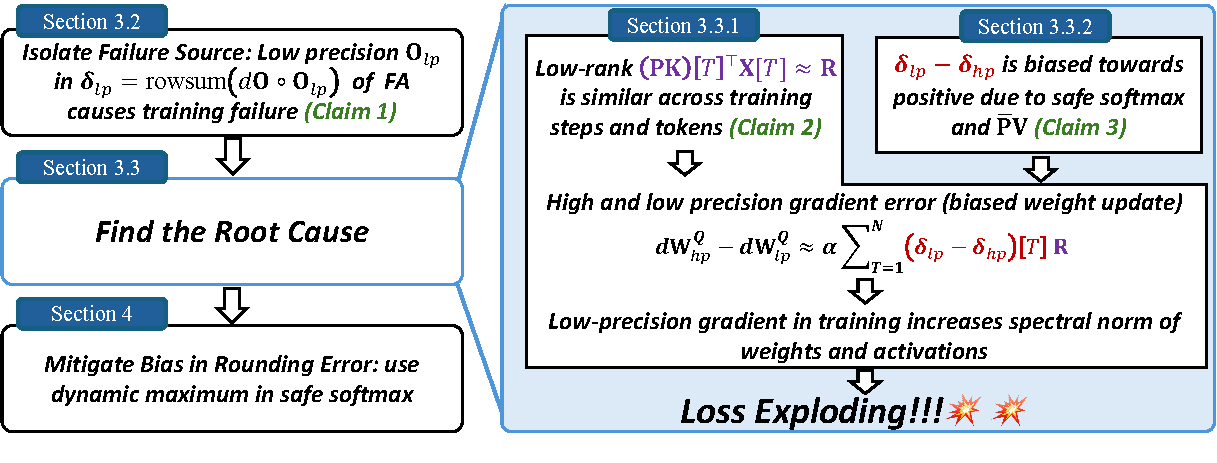
\includegraphics[width=\textwidth]{img/failure_process.pdf}
  \vspace{-10pt}
  \caption{各章节的分析概览。本文沿着训练失败（蓝框）的因果链逆向追踪，以识别根本原因。}\label{fig:failure_process}
  \vspace{-10pt}
\end{figure}


\section{Flash Attention 不稳定的根本原因}

我们首先在 \cref{ssec:failure_case} 介绍失败案例。
在 \cref{ssec:narrow} 中，我们缩小了 Flash Attention 中数值错误的来源。进一步在 \cref{ssec:root_cause} 的分析表明，失败源于两个因素的组合：低秩表示的出现和 BF16 算术中固有的有偏舍入误差的积累。此类故障从根本原因到损失爆炸的完整过程如 \cref{fig:failure_process} 所示。




\subsection{低精度 Flash Attention 的失败案例}\label{ssec:failure_case}
  
\begin{wrapfigure}{r}{0.4\textwidth}
  \vspace{-15pt}
    \centering
    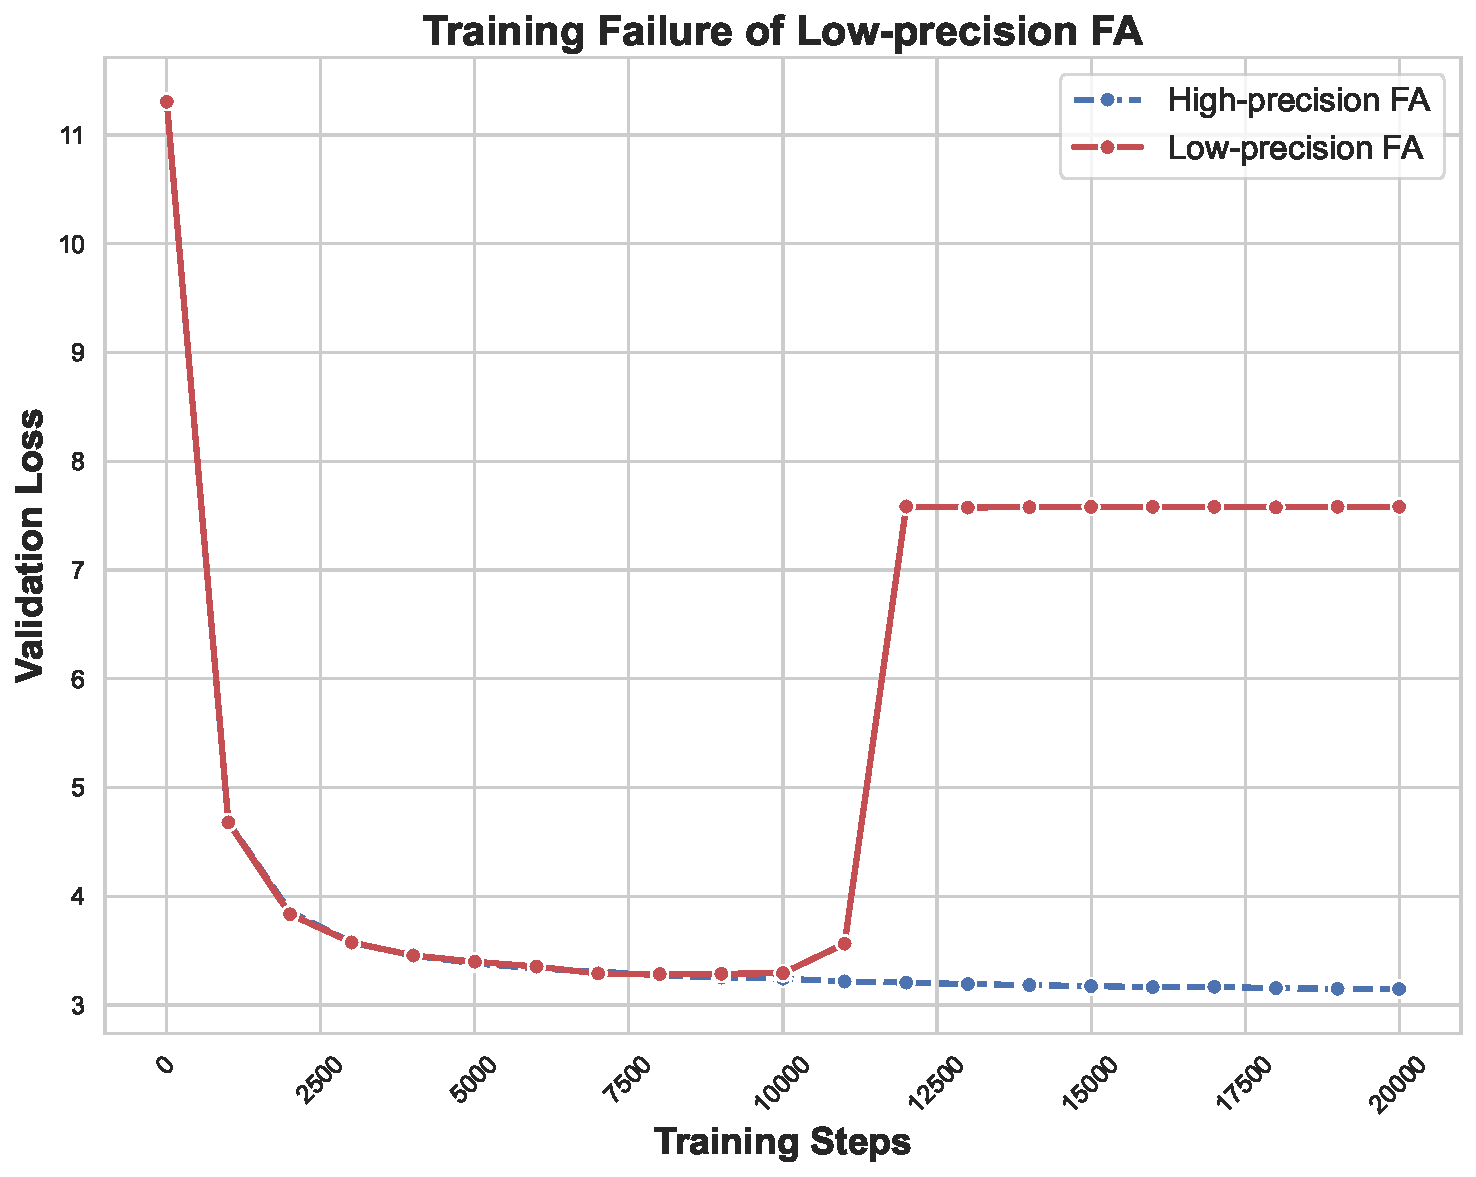
\includegraphics[width=0.4\textwidth]{img/stable_unstable_loss.pdf}
  \vspace{-20pt}
    \caption{使用 BF16 与 Flash Attention 的失败案例导致损失突然爆炸，而稳定配置则可收敛。}\label{fig:exploded_loss}
  \vspace{-10pt}
    % visualize_loss.py
\end{wrapfigure}

我们的调查针对的是一个有据可查且持续存在的故障：在以 BF16 精度训练使用 Flash Attention 的生成式预训练 Transformer 2 (GPT-2) 模型时发生的灾难性损失爆炸~\citep{nanogpt_issue303,nanogpt_issue524,nanogpt_issue554}。这个失败案例已经报告了两年多，表现为经过数千个训练步骤后突然出现损失爆炸（参见 \cref{fig:nanogpt_issues}）。虽然回退到标准注意力或使用更高精度（FP32）等经验性方案可以稳定训练，但它们以效率为代价。这种不稳定并不是孤立事件；更广泛的社区在训练大型语言模型时也观察到了类似失败~\citep{team2025kimi,qwen3technicalreport}。这些失败通常根据经验与权重谱范数大、激活大等现象相关~\citep{yang2023spectral,rybakov2024methods}，以及注意力沉陷~\citep{xiao2023efficient}，从而引发一系列修复，包括 QK 归一化~\citep{henry2020query,qwen3technicalreport}、QK 裁剪~\citep{team2025kimi} 和门控注意~\citep{qiu2025gated,qwen3technicalreport}。尽管采取了这些干预措施，但对根本原因的基本理解仍然缺失。缺乏从数值误差到损失爆炸的明确因果链，使社区依赖临时补丁而非原则性方案，从而阻碍了稳健低精度训练的进展。本文通过重现故障、剖析其根本原因并提出实用的原则性解决方案，提供了第一个机制性解释。



为了重现失败，我们采用了具有 12 层、12 个注意力头、嵌入维度为 768、上下文长度为 1024 的 GPT-2 架构。该模型是在 OpenWebText 数据集上进行预训练的~\citep{Gokaslan2019OpenWeb}. 
为了实现确定性的再现性，我们偏离了标准随机数据加载器，记录并重用了导致失败的初始运行中的数据批次的确切序列。 
这确保了所有后续实验以相同的顺序处理相同的数据，从而将失败与数据相关的随机性隔离开来。

我们使用 AdamW 优化器训练模型 $\beta_1=0.9$, $\beta_2=0.95$，并且重量衰减为零。 
学习率遵循余弦计划，通过 2000 次迭代线性预热达到峰值 $1 \times 10^{-3}$, 衰减到 $1 \times 10^{-5}$. 
我们应用最大范数为 1.0 的全局梯度裁剪。 
使用 PyTorch 的分布式数据并行 (DDP) 模块在 4 个 NVIDIA A100 (80GB) GPU 上进行训练。 
我们使用自动混合精度，BF16 用于前向传递，FP32 用于后向传递。 
每个 GPU 处理的微批量大小为 32，并且梯度累积超过 4 个步骤， 
每个优化步骤的有效全局批量大小为 524,288 个令牌。

\subsection{在 Flash Attention 中隔离故障源}\label{ssec:narrow}

为了查明 Flash Attention 失败的根源，我们进行了一系列有针对性的实验。我们系统地修改算法——禁用平铺、有选择地用标准实现替换 Flash Attention、并以高精度执行关键计算——以缩小不稳定的潜在原因。为了加速这一分析，我们监控权重谱范数等经验指标，以快速识别失败配置。


\vspace{-10pt}
\paragraph{平铺不是失败的根源。}
为了确定 Flash Attention 中的分块处理是否是导致失败的原因，我们进行了一项实验，通过将块大小设置为等于序列长度来禁用平铺。这迫使算法立即使用完整的矩阵进行计算。训练过程仍然失败，导致同样的损失爆炸。这一发现排除了平铺策略是导致问题的原因。因此，对于所有后续实验，我们使用这种非平铺设置来简化分析并专注于核心数值计算。

\vspace{-10pt}
\paragraph{故障源于单层。}
我们首先分析各层权重的谱范数~\citep{yang2023spectral,rybakov2024methods}. 
这揭示了第二层注意力中的异常尖峰（参见 \cref{fig:sp_norm}). 
我们通过两个有针对性的实验证实了这一发现： 
(1) 仅在第 2 层使用 Flash Attention 就足以重现训练失败，并且 
（2）在第 2 层用标准注意力替换 Flash Attention，同时在所有其他层中保留它，恢复了训练的稳定性。 
这些结果最终确定了第 2 层中的 Flash Attention 是失败的根源。因此，后续分析主要围绕该模块来剖析故障机制。

\vspace{-10pt}
\paragraph{失败与 $\rvdel$ 的计算有关。} Flash Attention 的反向传播使用 $\rvdel = \mathrm{rowsum}(d\rmO \circ \rmO)\in \mathbb{R}^{N}$ 来提高计算效率。另一种数学上等效的公式将该项计算为 $\rvdel = \mathrm{rowsum}(d\rmP \circ \rmP)$，其中 $d\rmP = d\rmO \rmV^\top$。我们发现用这种替代公式替换原有计算可以恢复训练稳定性。该实验表明，BF16 计算 $\rmO$ 时引入的数值误差可能是失败的主要来源，因为该替代公式等效于在 FP32 中使用 $\rmO$。
\begin{wrapfigure}{r}{0.4\textwidth}
    \centering
    % \vspace{-10px}
    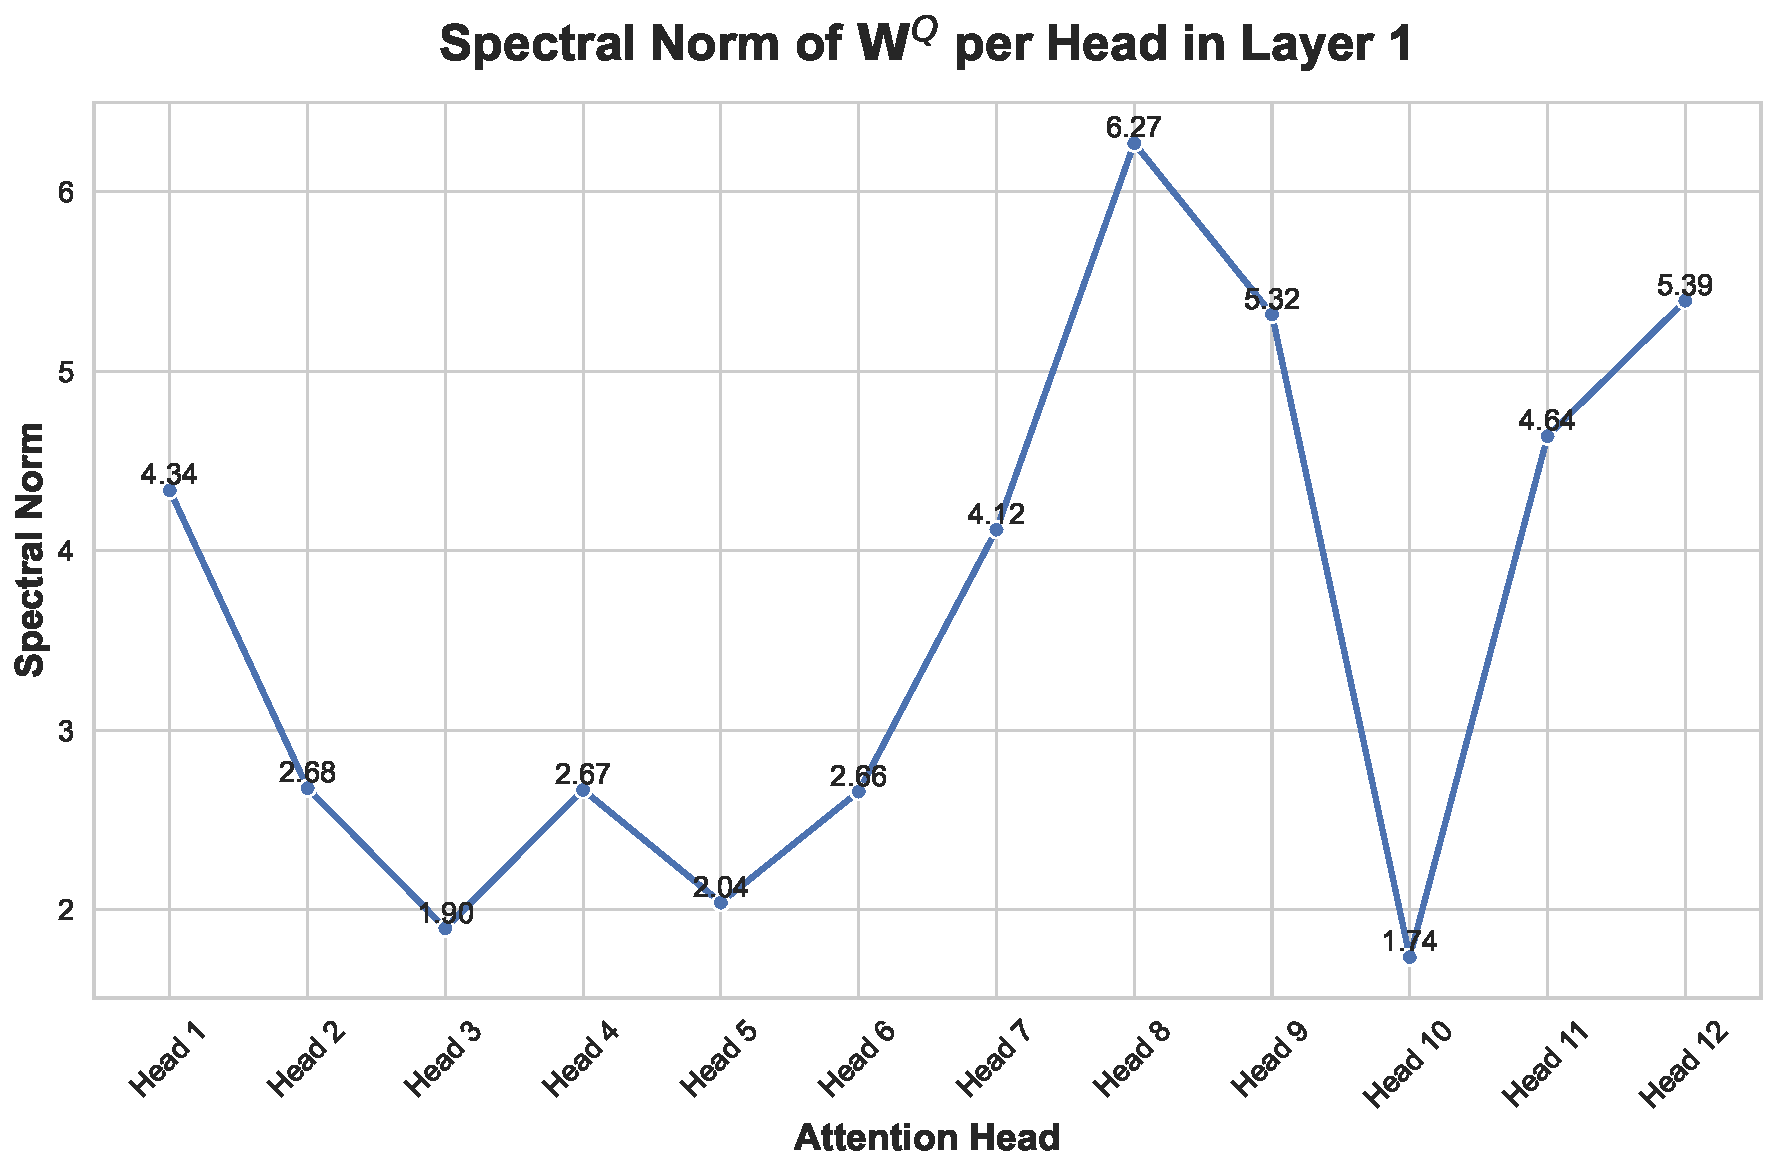
\includegraphics[width=0.4\textwidth]{img/layer_1_wq_head_spectral_norms.pdf}
    \vspace{-20pt}
    \caption{注意力头 8 的 $\rmW^Q$ 具有最大的谱范数，后续分析聚焦于该头。}\label{fig:head_locating}
    \vspace{-20pt}
    % visualize_head8_sp.py
\end{wrapfigure}

\vspace{-10pt}
\paragraph{$\rmO$ 中的数值误差是失败的根源。}
基于以下发现：计算 $\rvdel$ 至关重要，我们进一步将误差源隔离到输出矩阵 $\rmO_{lp}$ 低精度 $\rvdel_{lp} = \mathrm{rowsum}(d\rmO \circ \rmO_{lp})$。我们进行了两个关键实验。首先，不使用低精度 $\rmO$ 从前向传递到计算 $\rvdel$，我们将其重新计算为 $\rmP\rmV$ 在 FP32 内向后传递；这一变化稳定了训练。其次，我们发现计算 $\rmO$ 在前向传播过程中以高精度（FP32），即 $\rvdel_{hp} = \mathrm{rowsum}(d\rmO \circ \rmO_{hp})$在保留BF16所有其他操作的同时，也恢复了稳定性。这一证据最终证明了 BF16 计算过程中引入的数值误差 $\rmO$ 是导致故障的直接原因（参见 \cref{claim1}).


\vspace{-10pt}
\paragraph{失败被定位到特定的注意力头。}为了进一步缩小失败的来源，我们通过跟踪查询投影矩阵（$\rmW^Q$）的谱范数~\citep{yang2023spectral,rybakov2024methods}来分析各个注意力头，如 \cref{fig:head_locating} 所示。这表明一些注意力头表现出不成比例的谱范数。我们通过有选择地计算这些离群头（1、7、8、9、11 和 12）的高精度输出 $\rmO$ 来确认它们的作用，这足以恢复训练稳定性。\emph{由于头 8 显示了最大的谱范数，因此我们将后续分析集中在该头上，以剖析精确的故障机制。}


\begin{tcolorbox}[
  colback=cyan!5!white,
  colframe=black!100,
  boxrule=0.4pt,
  arc=3pt,
  left=5pt, right=5pt,
  top=5pt, bottom=5pt,
  width=0.95\linewidth,
  coltitle=black,
  center
]
\begin{claim}\label{claim1}
低精度 $\rvdel_{lp} = \mathrm{rowsum}(d\rmO \circ \rmO_{lp})$ 导致训练失败。
\end{claim}
% $\rvdel_{hp} = \mathrm{rowsum}(d\rmO \circ \rmO_{hp})$ in the backward of flash attention restores training stability.
\end{tcolorbox}

% \vspace{-5px}


\subsection{训练失败的根本原因}\label{ssec:root_cause}


我们在本节中的调查揭示了训练失败的两个相互关联的根本原因。在 \cref{ssec:cause1}，我们演示了低精度如何 $\rvdel_{lp}$ 通过有偏差的权重更新来驱动训练失败，并发现偏差是由于类似的低秩表示的出现而产生的 $\rmR$，其系数 $(\rvdel_{lp} - \rvdel_{hp})[T]$ 偏向正值，导致误差累积而不是抵消。在 \cref{ssec:cause2}，我们追踪这些正系数的起源 $(\rvdel_{lp} - \rvdel_{hp})[T]$ BF16 加法中固有的偏差舍入误差 $\bar{\rmP}\rmV$ 产品。

\subsubsection{原因 1. 类似的低秩矩阵偏差权重更新}\label{ssec:cause1}

本节将训练失败追溯到有偏差的权重更新。我们首先分析高低精度梯度计算的差异 $\rvdel_{hp}$ 和 $\rvdel_{lp}$， 分别。然后我们发现低秩表示和有偏差 $(\rvdel_{lp} - \rvdel_{hp})[T]$ 导致损失爆炸。

% \vspace{-5px}
\paragraph{高精度和低精度梯度之间的误差分析}为了了解数值误差如何传播到梯度中，我们分析了查询矩阵 $d\rmQ$ 的高精度 ($hp$) 和低精度 ($lp$) 梯度之间的差异。梯度 $d\rmQ$ 是根据注意力分数 $d\rmS$ 的梯度计算出来的，如 $d\rmQ = d\rmS \rmK$。分数梯度由 $d\rmS = \alpha \rmP \circ (d\rmP - \rvdel)$ 给出，其中 $\rvdel = \mathrm{rowsum}(d\rmO \circ \rmO)$ 是基于 \cref{ssec:narrow} 中高精度与低精度反向传递之间唯一不同的项，且 $\alpha$ 是注意力的比例因子。

高精度和低精度查询梯度之间的差异可以推导为：
% \vspace{-5px}
\begin{equation}\label{eq:q_diff}
  \begin{split}
  & d\rmQ_{hp} - d\rmQ_{lp} = (d\rmS_{hp} - d\rmS_{lp})\rmK \\
  =& \left( \alpha \rmP \circ (d\rmP - \rvdel_{hp}) - \alpha \rmP \circ (d\rmP - \rvdel_{lp}) \right) \rmK
  = \left( \alpha \rmP \circ (\rvdel_{lp} - \rvdel_{hp}) \right) \rmK \\
  =& \alpha \cdot \mathrm{diag}(\rvdel_{lp} - \rvdel_{hp}) (\rmP \rmK).
  \end{split}
% \vspace{-5px}
\end{equation}
在最后一步中，我们表达逐行缩放操作 $\rmP \circ (\rvdel_{lp} - \rvdel_{hp})$ （遵循广播规则）作为矩阵乘法，其中 $\mathrm{diag}(\rvdel_{lp} - \rvdel_{hp})$  是一个对角矩阵，其对角元素是向量差的元素 $\rvdel_{lp} - \rvdel_{hp}$。该公式表明梯度误差与误差成正比 $\rvdel$ 并由术语调制 $\rmP \rmK$.


\begin{figure}[t]
  \centering
  \subfigure[]{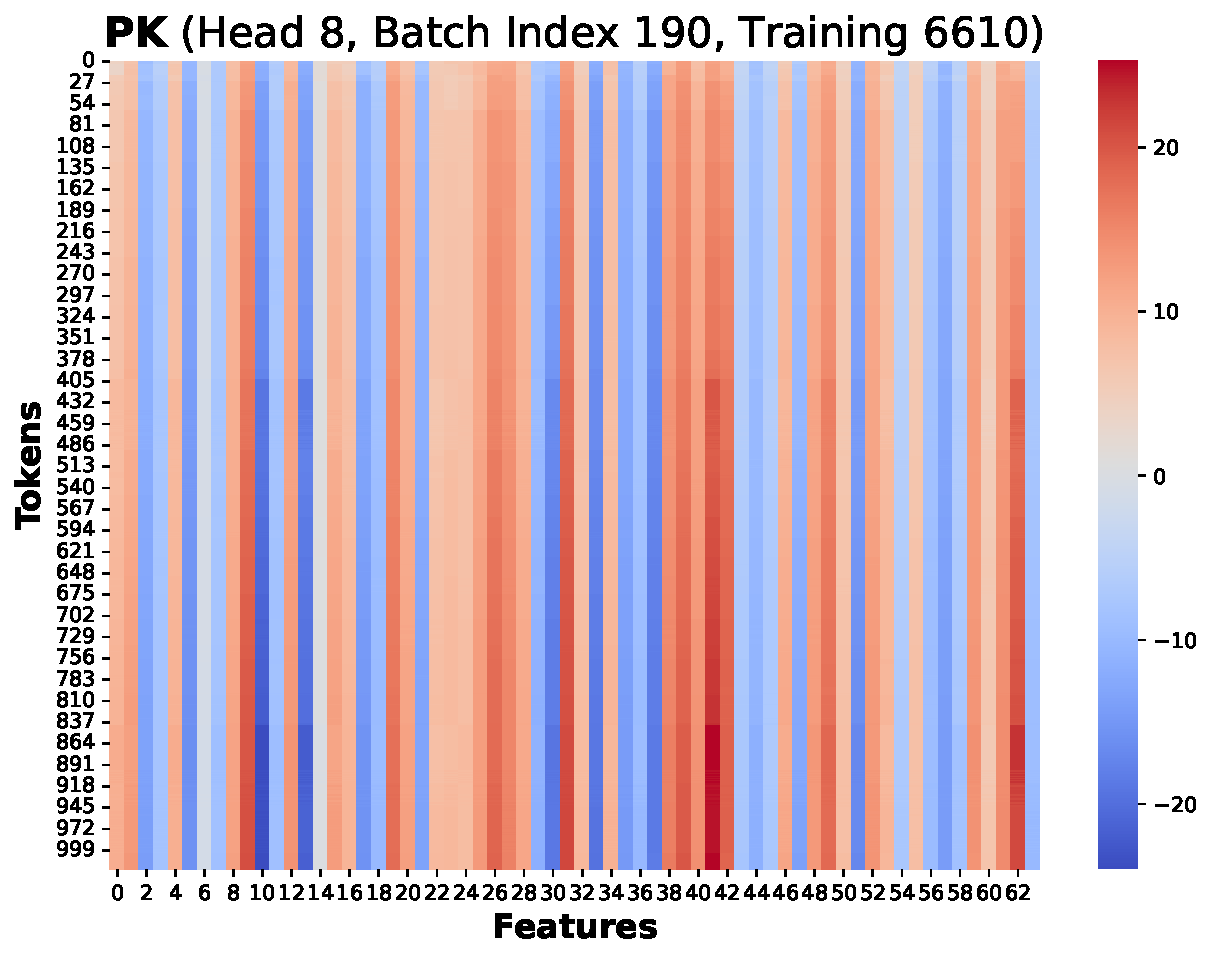
\includegraphics[width=0.3\textwidth]{img/PK_at_H8_batch_idx_190_6610.pdf}}
  \subfigure[]{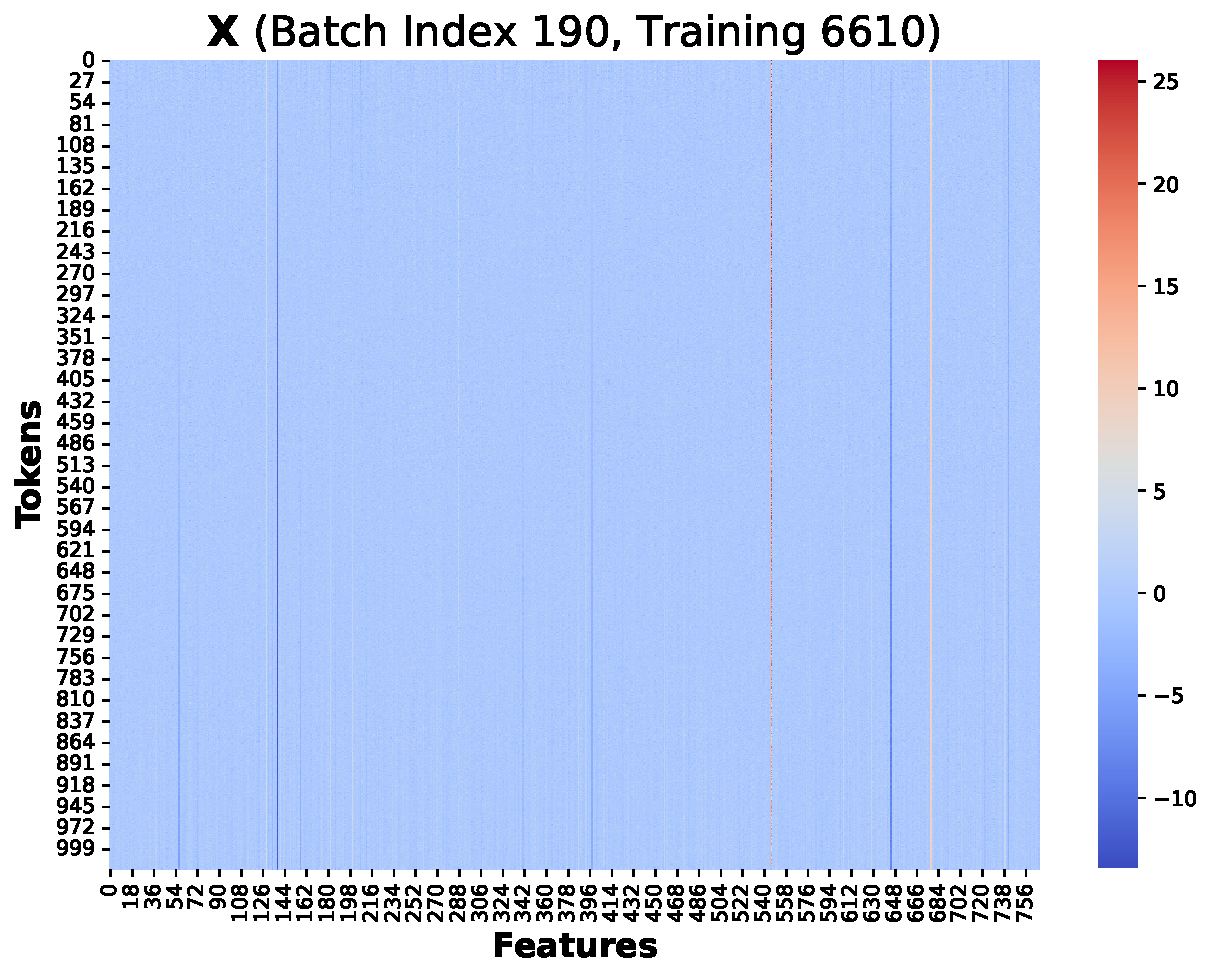
\includegraphics[width=0.3\textwidth]{img/X_at_batch_idx_190_train_steps_6610.pdf}}
  \subfigure[]{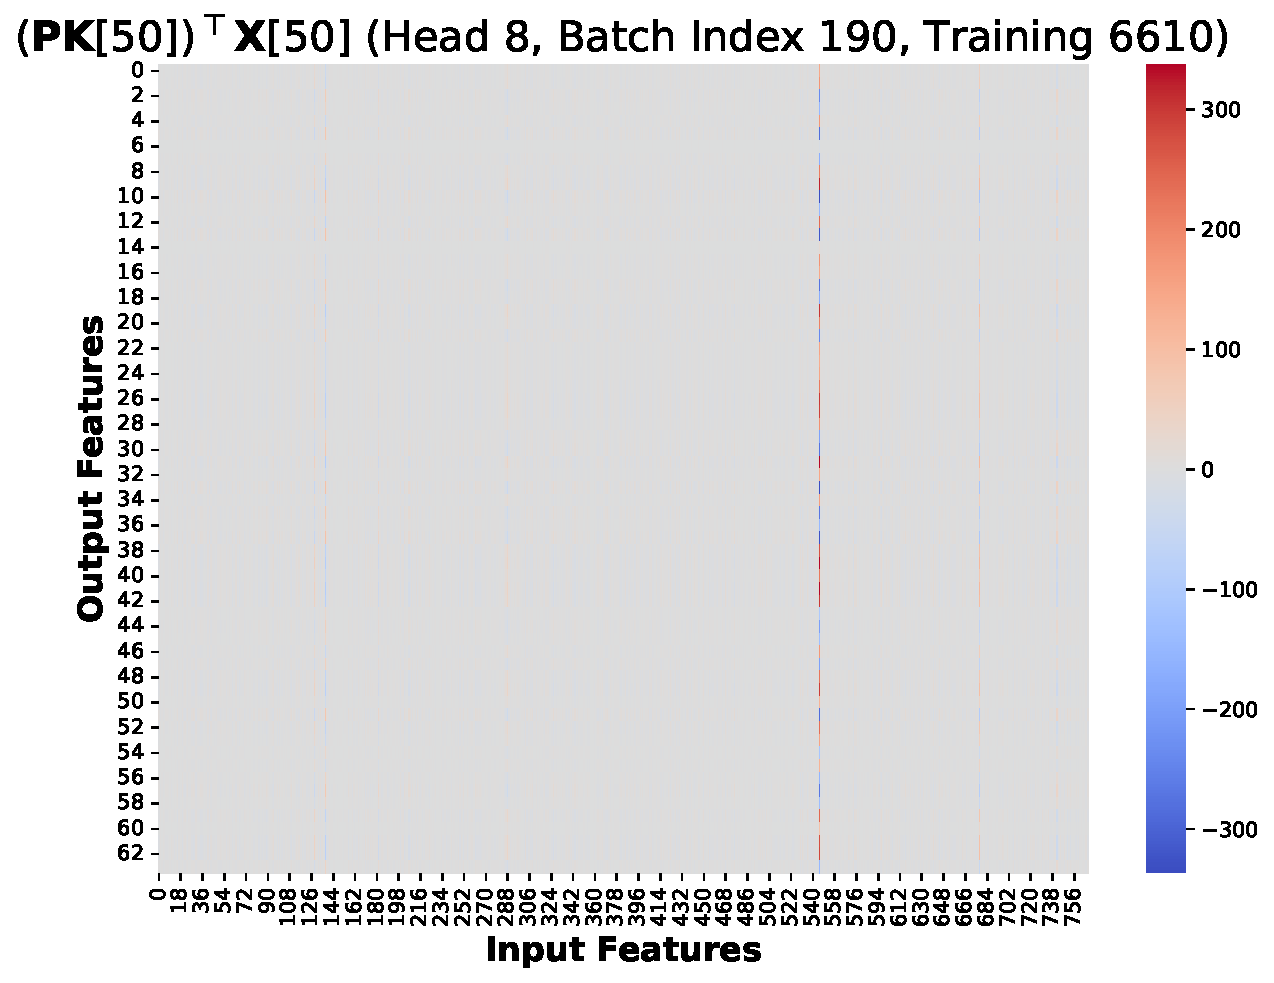
\includegraphics[width=0.3\textwidth]{img/PKX_at_H8_batch_idx_190_token50_train_steps_6610.pdf}}
  \subfigure[]{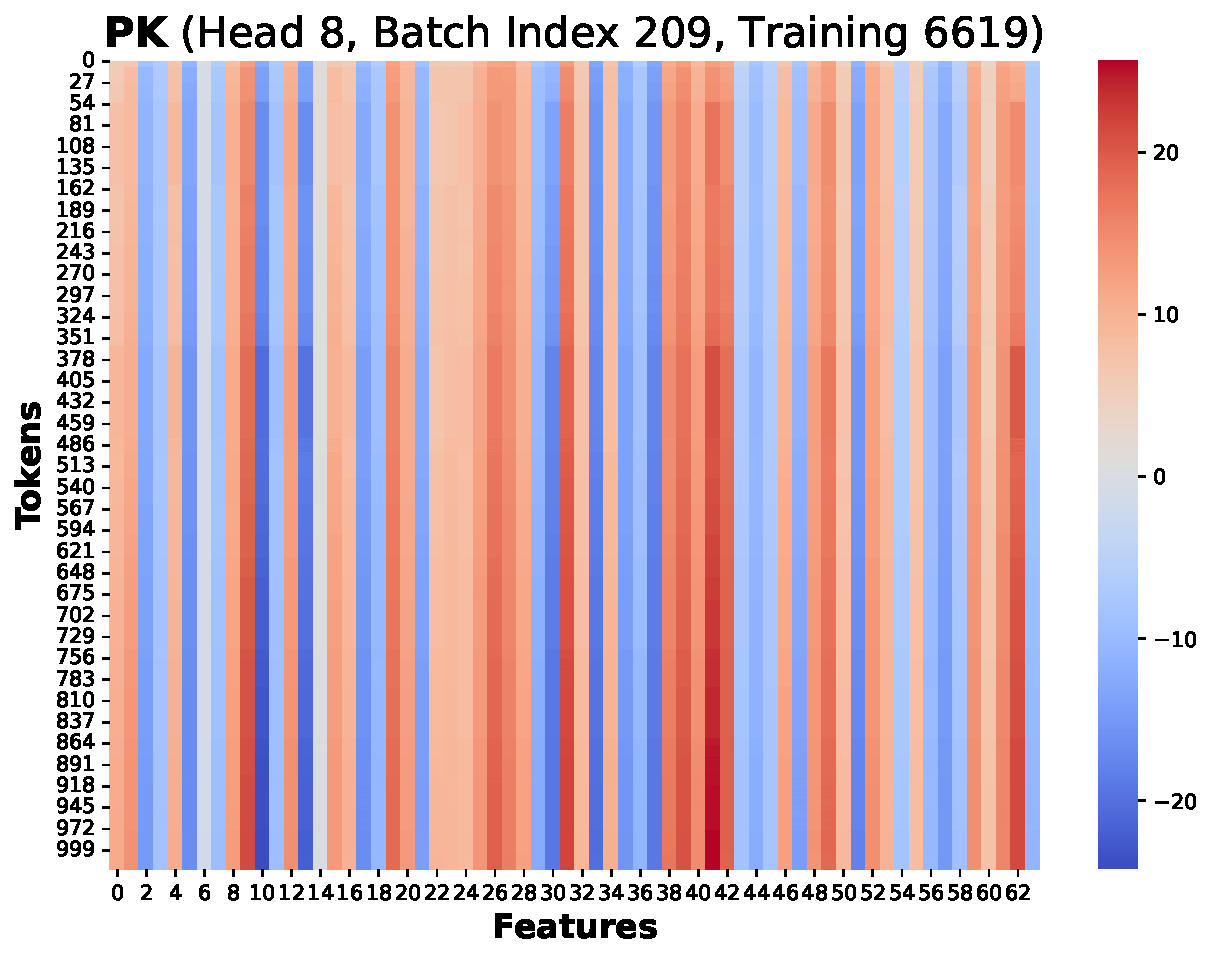
\includegraphics[width=0.3\textwidth]{img/PK_at_H8_batch_idx_209_6619.pdf}}
  \subfigure[]{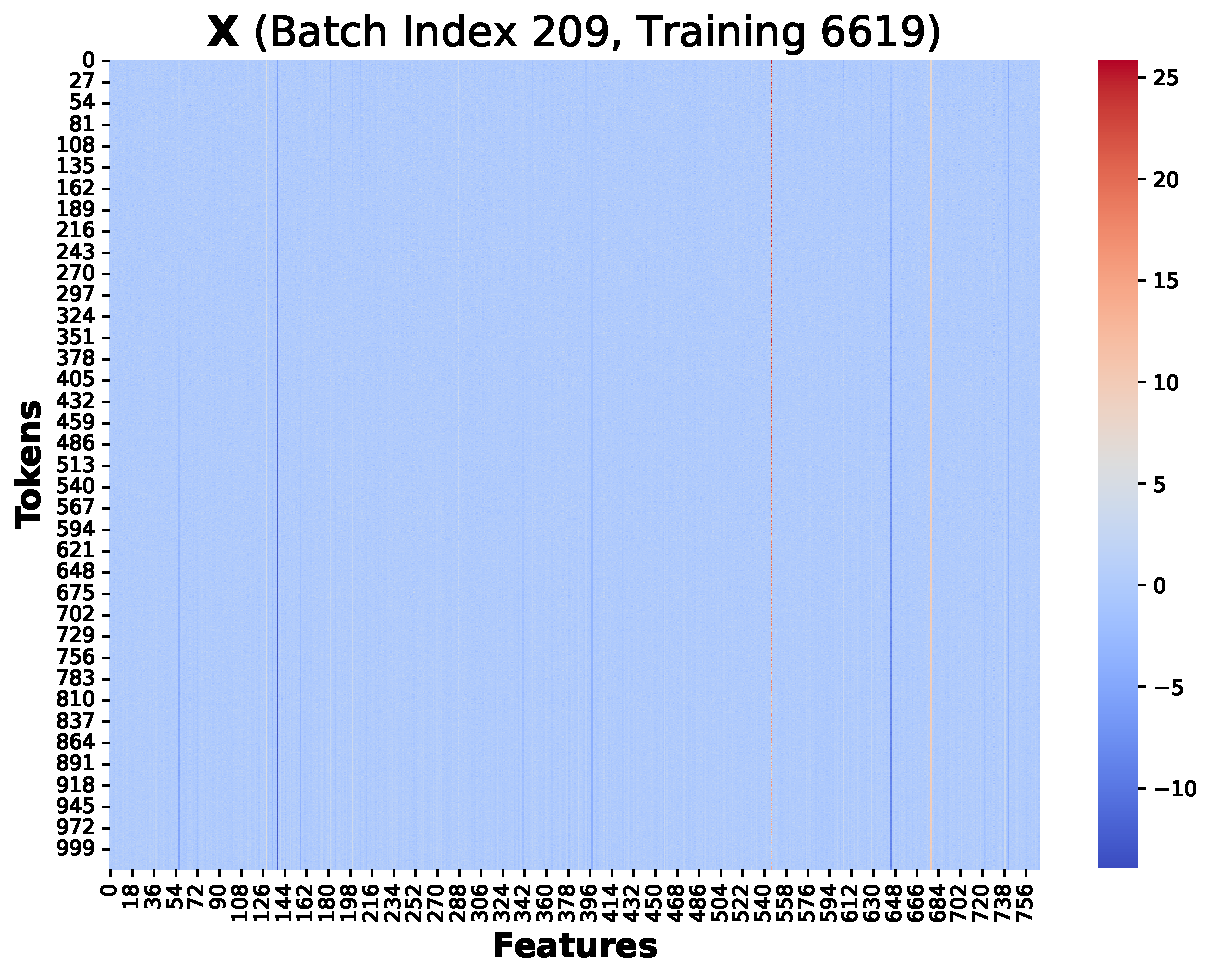
\includegraphics[width=0.3\textwidth]{img/X_at_batch_idx_209_train_steps_6619.pdf}}
  \subfigure[]{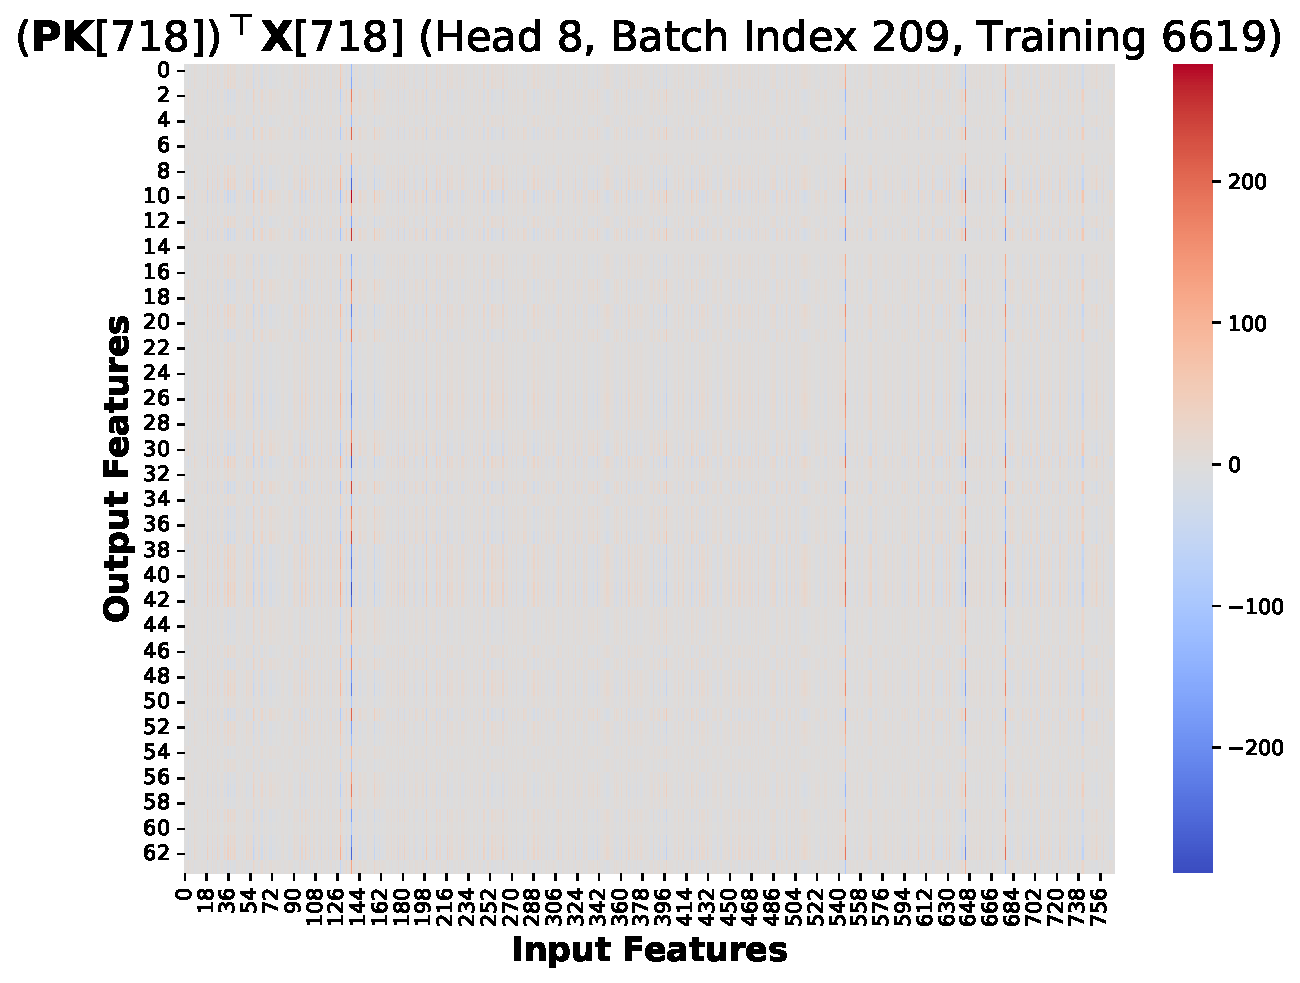
\includegraphics[width=0.3\textwidth]{img/PKX_at_H8_batch_idx_209_token718_train_steps_6619.pdf}}
  \vspace{-10pt}
  \caption{$\rmP \rmK$, $\rmX$, and $(\rmP \rmK)[T]^\top \rmX[T]$ at different batch indices and training steps. (c) and (f) show that $(\rmP \rmK)[T]^\top \rmX[T]$ for different tokens and training steps have some similar columns in input features 546 and 678.}\label{fig:vis_PK_X}
  \vspace{-15pt}
  %  matrix_alignment_v2.ipynb plots PK
  %  train_one_sample.ipynb saves the state for plotting PK
  %  train_one_sample.ipynb plots X
\end{figure}


查询投影矩阵的梯度， $d\rmW^Q$，由输入特征的外积给出 $\rmX$ 和查询梯度 $d\rmQ$。高精度之间的差异（$hp$）和低精度（$lp$) 的梯度 $\rmW^Q$ 可以表示为：
% \vspace{-5px}
\begin{align}
d\rmW^Q_{hp} - d\rmW^Q_{lp} 
& = (d\rmQ_{hp} - d\rmQ_{lp})^\top \rmX
=  \alpha (\rmP \rmK)^\top \mathrm{diag}(\rvdel_{lp} - \rvdel_{hp}) \rmX,
\notag\\
& = \alpha \sum\nolimits_{T=1}^N (\rvdel_{lp} - \rvdel_{hp})[T] \cdot (\rmP \rmK)[T]^\top \rmX[T],
\label{eq:grad_diff}
% \vspace{-5px}
\end{align}
在哪里 $(\rmP \rmK)[T]$ 和 $\rmX[T]$ 是 $T$其矩阵的第行向量。该方程表明总梯度误差是 1 阶矩阵的加权和，权重由误差给出 $\rvdel$.


% \vspace{-5px}
\paragraph{权重的类似低秩更新导致训练失败}在\cref{fig:vis_PK_X}中，$\rmP\rmK$（面板a，d）和$\rmX$（面板b，e）的行在不同的训练步骤和令牌位置上表现出很强的结构相似性。这意味着生成的 1 阶矩阵 $(\rmP \rmK)[T]^\top \rmX[T]$ 也彼此高度相似。例如，\cref{fig:vis_PK_X} (图c、f)分别示出了在训练步骤6610和6619处标记50和718的这种相似性。由于这些 1 级误差分量在结构上是一致的，因此我们可以将总梯度差近似为 
\begin{equation}\label{eq:low_rank_approx}
  d\rmW^Q_{hp} - d\rmW^Q_{lp} \approx \alpha \sum\nolimits_{T=1}^N (\rvdel_{lp} - \rvdel_{hp})[T] \rmR
\end{equation}
在哪里 $\rmR$ 表示不同令牌和训练步骤中出现的常见低等级结构。

等式（\ref{eq:low_rank_approx})表明低秩误差方向的累积 $\rmR$ 由标量项控制 $\sum_{T=1}^N (\rvdel_{lp} - \rvdel_{hp})[T]$。如果该总和偏向于非零值，则不同训练步骤的误差将累积而不是抵消。我们跟踪累计总和 $\sum_{T=1}^N (\rvdel_{lp} - \rvdel_{hp})[T]$ 通过一系列训练步骤（6580 到 6680）导致失败，如图所示 \cref{fig:D_do_o_analysis}（一个）。该图显示该总和始终为正，表明存在系统偏差。这种偏差导致低秩方向的误差 $\rmR$ 与每个训练步骤相结合。因为 $\rmR$ 对于不同的步骤也类似，这最终会破坏权重更新，增加谱范数（\cref{fig:sp_norm}）和激活~\citep{yang2023spectral,rybakov2024methods}，并导致训练失败（参考 \cref{claim2}）。以下部分通过分析训练步骤 6619 中的权重和梯度找到了这种正偏差的根本原因，这是在 \cref{fig:D_do_o_analysis}(a).


\begin{tcolorbox}[
  colback=cyan!5!white,
  colframe=black!100,
  boxrule=0.4pt,
  arc=3pt,
  left=5pt, right=5pt,
  top=5pt, bottom=5pt,
  width=0.95\linewidth,
  coltitle=black,
  center
]
\begin{claim}\label{claim2}
  低精度训练中的权重更新存在偏差 $(\rvdel_{lp} - \rvdel_{hp})[T]\rmR$，它由结构相似的矩阵产生（表示为 $\rmR$）跨令牌和训练步骤，及其正偏系数 $(\rvdel_{lp} - \rvdel_{hp})[T]$。这种偏差会累积误差，防止抵消，增加权重谱范数和激活，并导致损失爆炸。
\end{claim}
\end{tcolorbox}


\begin{figure}[ht]
  % \vspace{-10px}
  \subfigure[{Positively-biased $(\rvdel_{lp} \!-\! \rvdel_{hp})[T]$}]{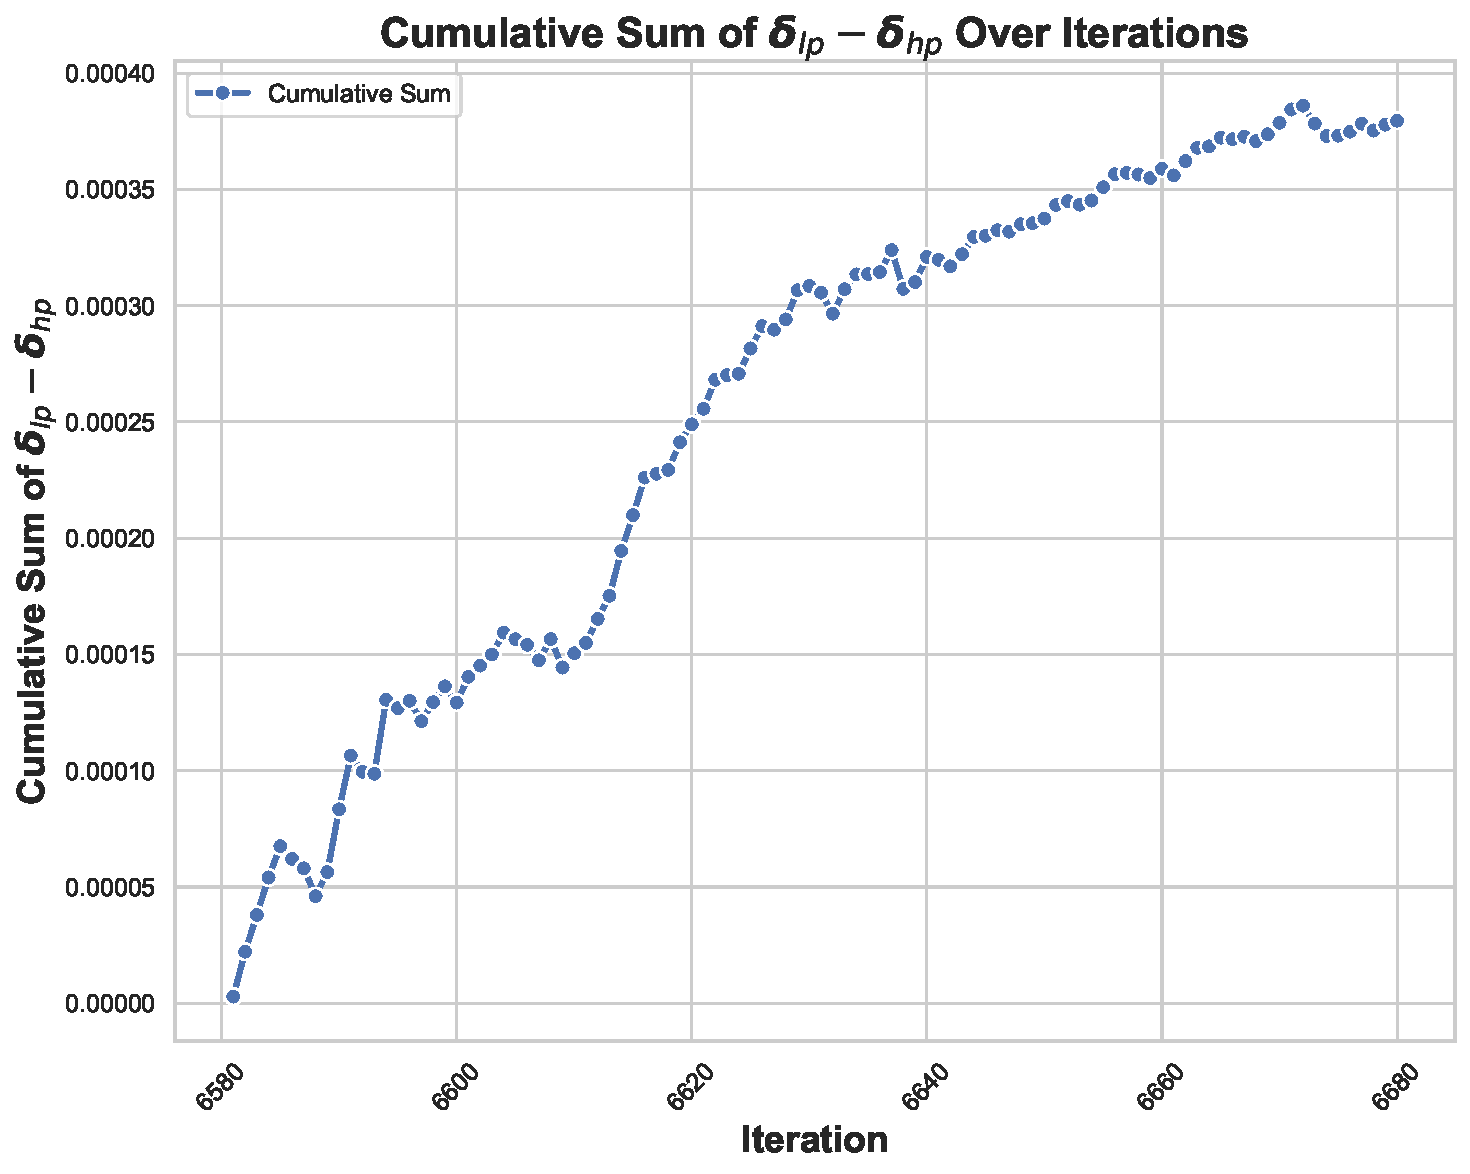
\includegraphics[width=0.32\textwidth]{img/cumsum_of_D_diff.pdf}}
  \subfigure[{特征 20 与 29 中的较大值}]{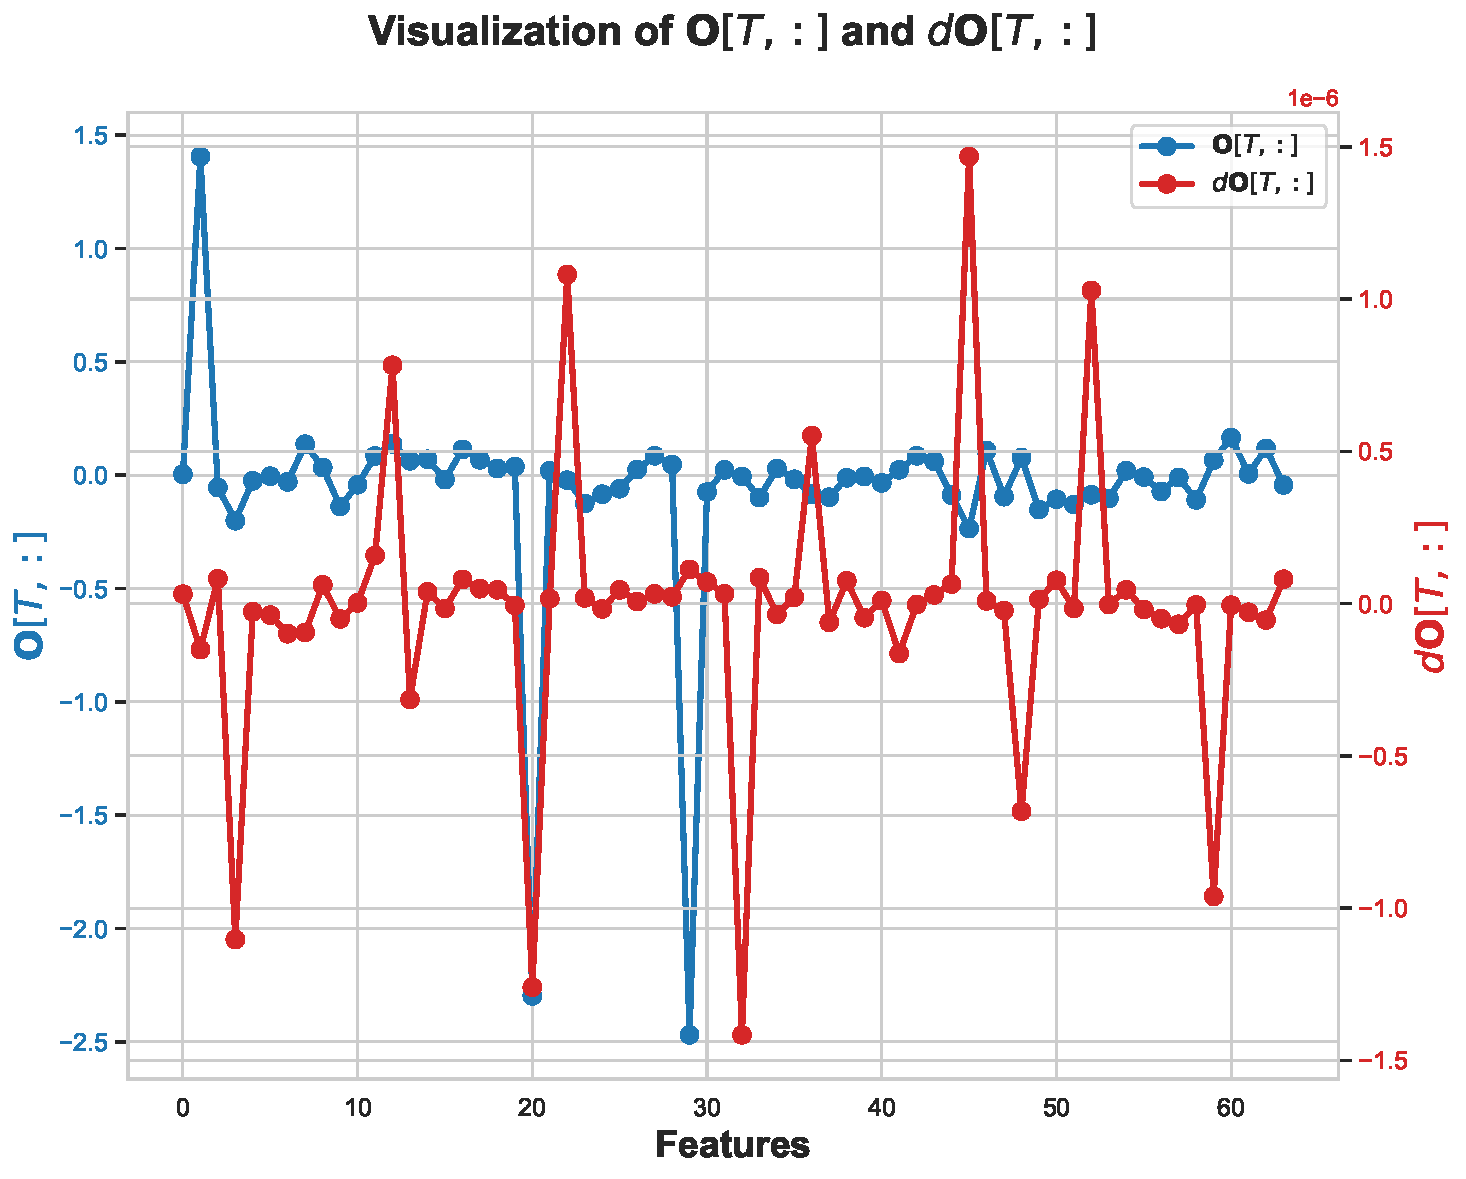
\includegraphics[width=0.32\textwidth]{img/o_do_visualization.pdf}}
  \subfigure[{特征 20 与 29 中的较大误差}]{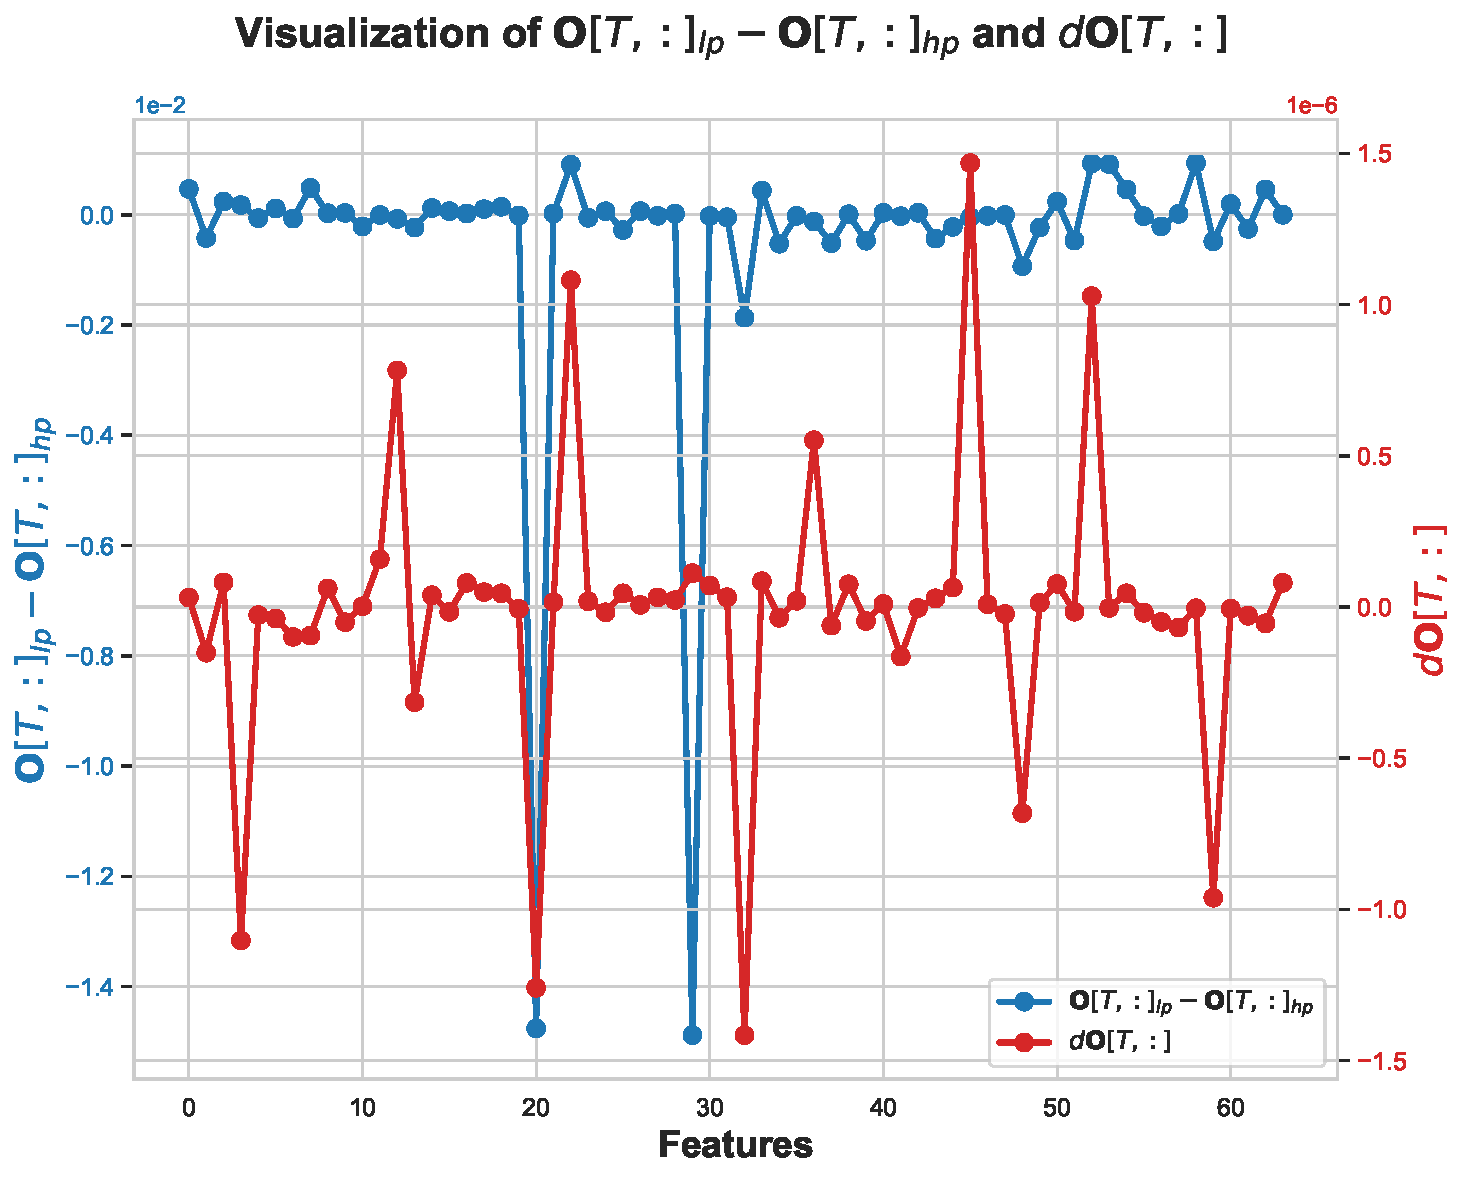
\includegraphics[width=0.32\textwidth]{img/o_diff_do_visualization.pdf}}
  \vspace{-10pt}
  \caption{分析 $\rvdel=\mathrm{rowsum}(d\rmO \circ \rmO)$.}\label{fig:D_do_o_analysis}
  % \vspace{-20px}
    % do_o_sample_analysis.ipynb
\end{figure}



% \vspace{-10px}
\subsubsection{原因 2. 有偏差的舍入误差导致正 \texorpdfstring{$(\rvdel_{lp} - \rvdel_{hp})[T]$}{}}\label{ssec:cause2}

本节研究了积极偏见的起源 $(\rvdel_{lp} - \rvdel_{hp})[T]$。我们将这个错误追溯到之间的相互作用 $d\rmO$ 以及数值上的差异 $\rmO_{lp} - \rmO_{hp}$，其本身是由于 BF16 加法过程中的舍入偏差产生的 $\bar{\rmP}\rmV$ 计算。

\begin{figure}[t]
  % \vspace{-10px}
    \centering
    \subfigure[{$\rmV[:, i]$ 多为负值}]{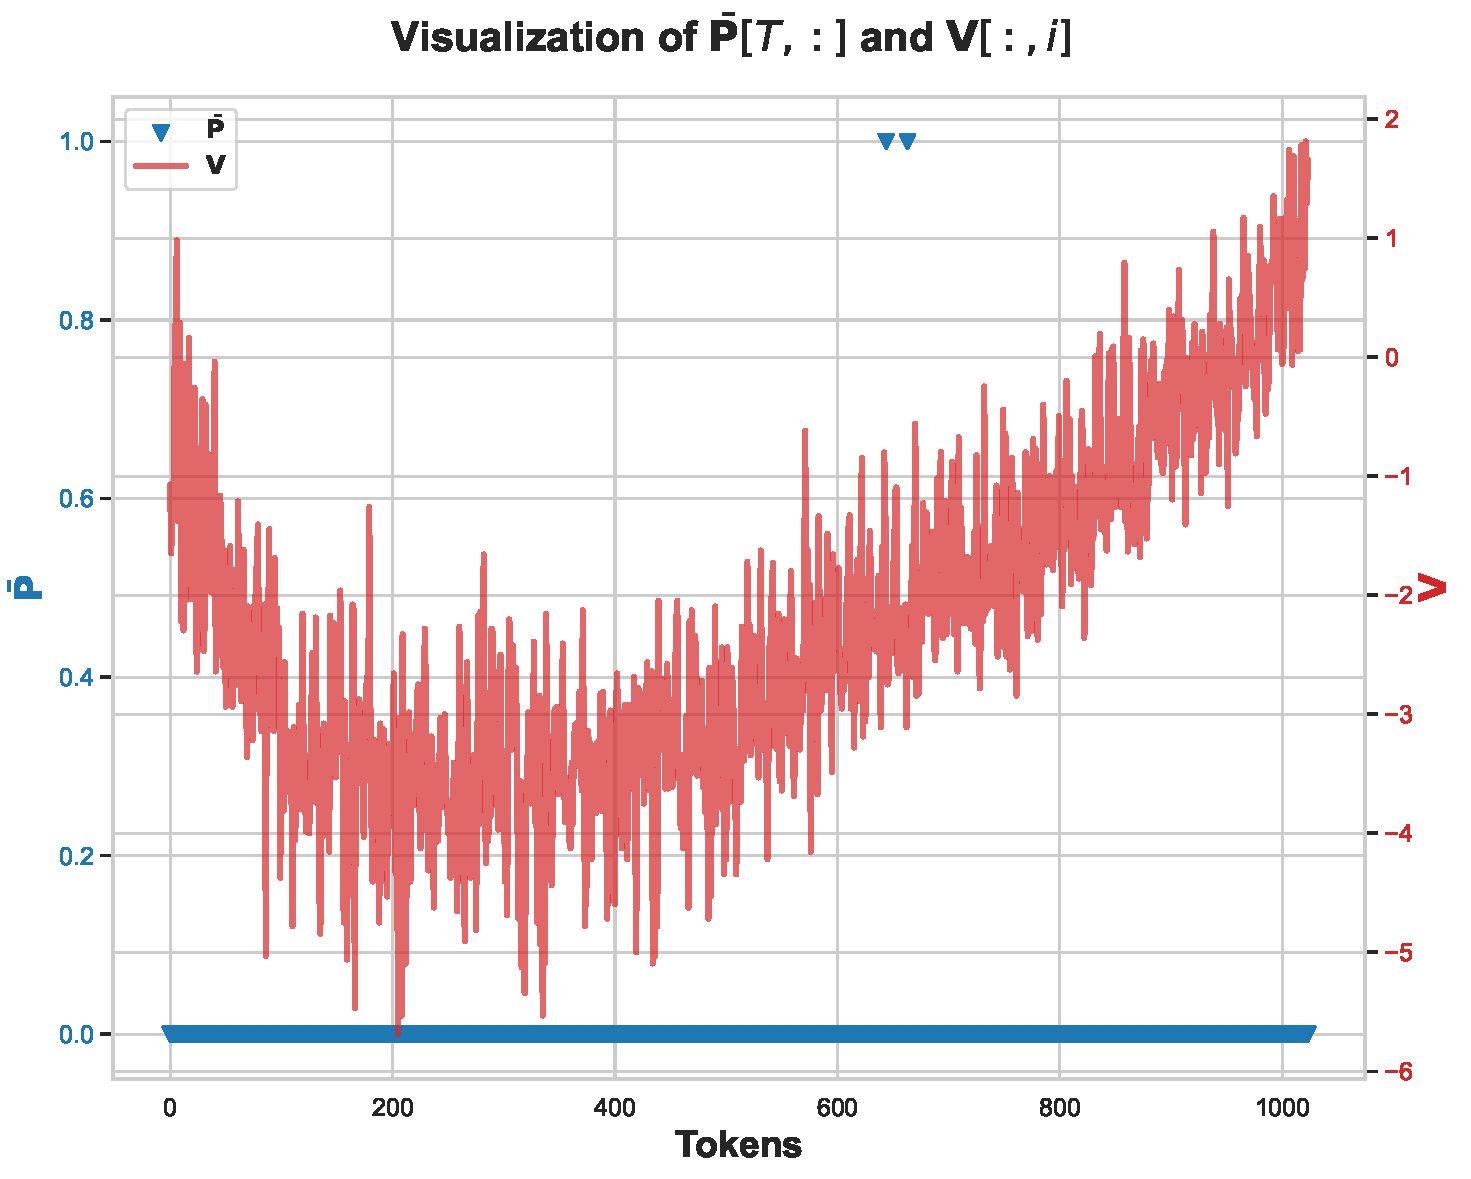
\includegraphics[width=0.32\textwidth]{img/P_V_visualization.pdf}}
    \subfigure[{$\bar{\rmP}[T, i]=1$ 时误差较大}]{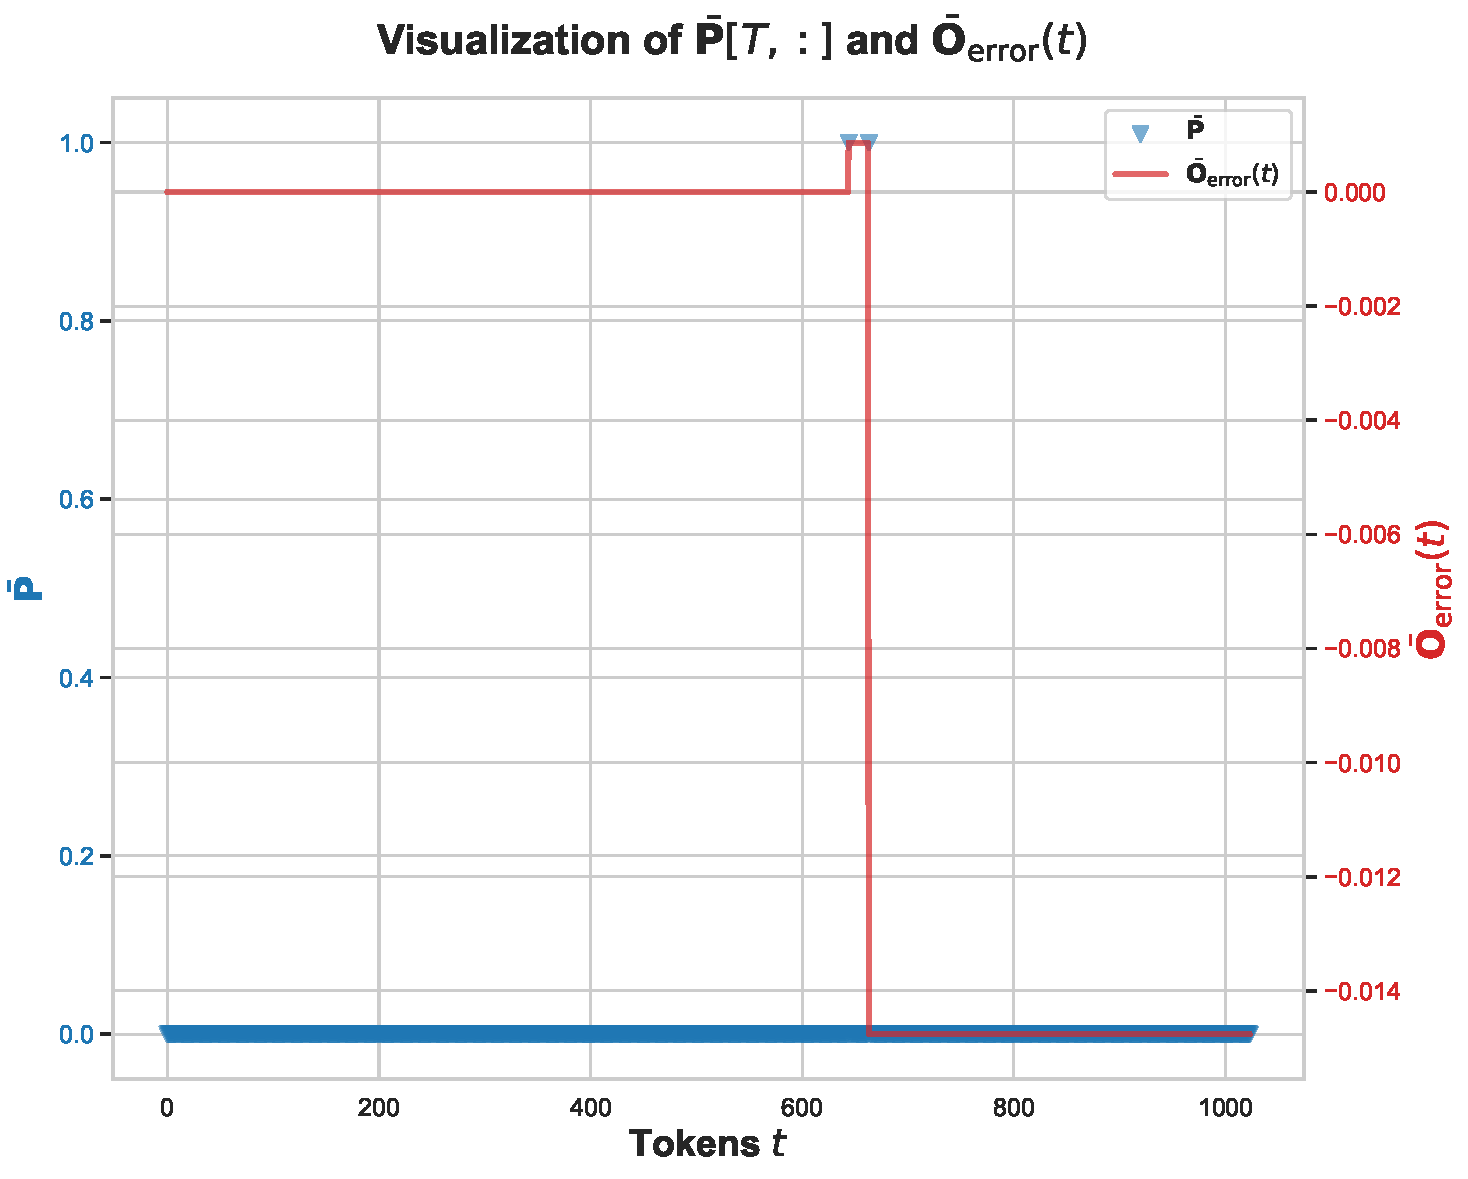
\includegraphics[width=0.32\textwidth]{img/o_error_visualization.pdf}}
    \subfigure[{(b) 的局部放大}]{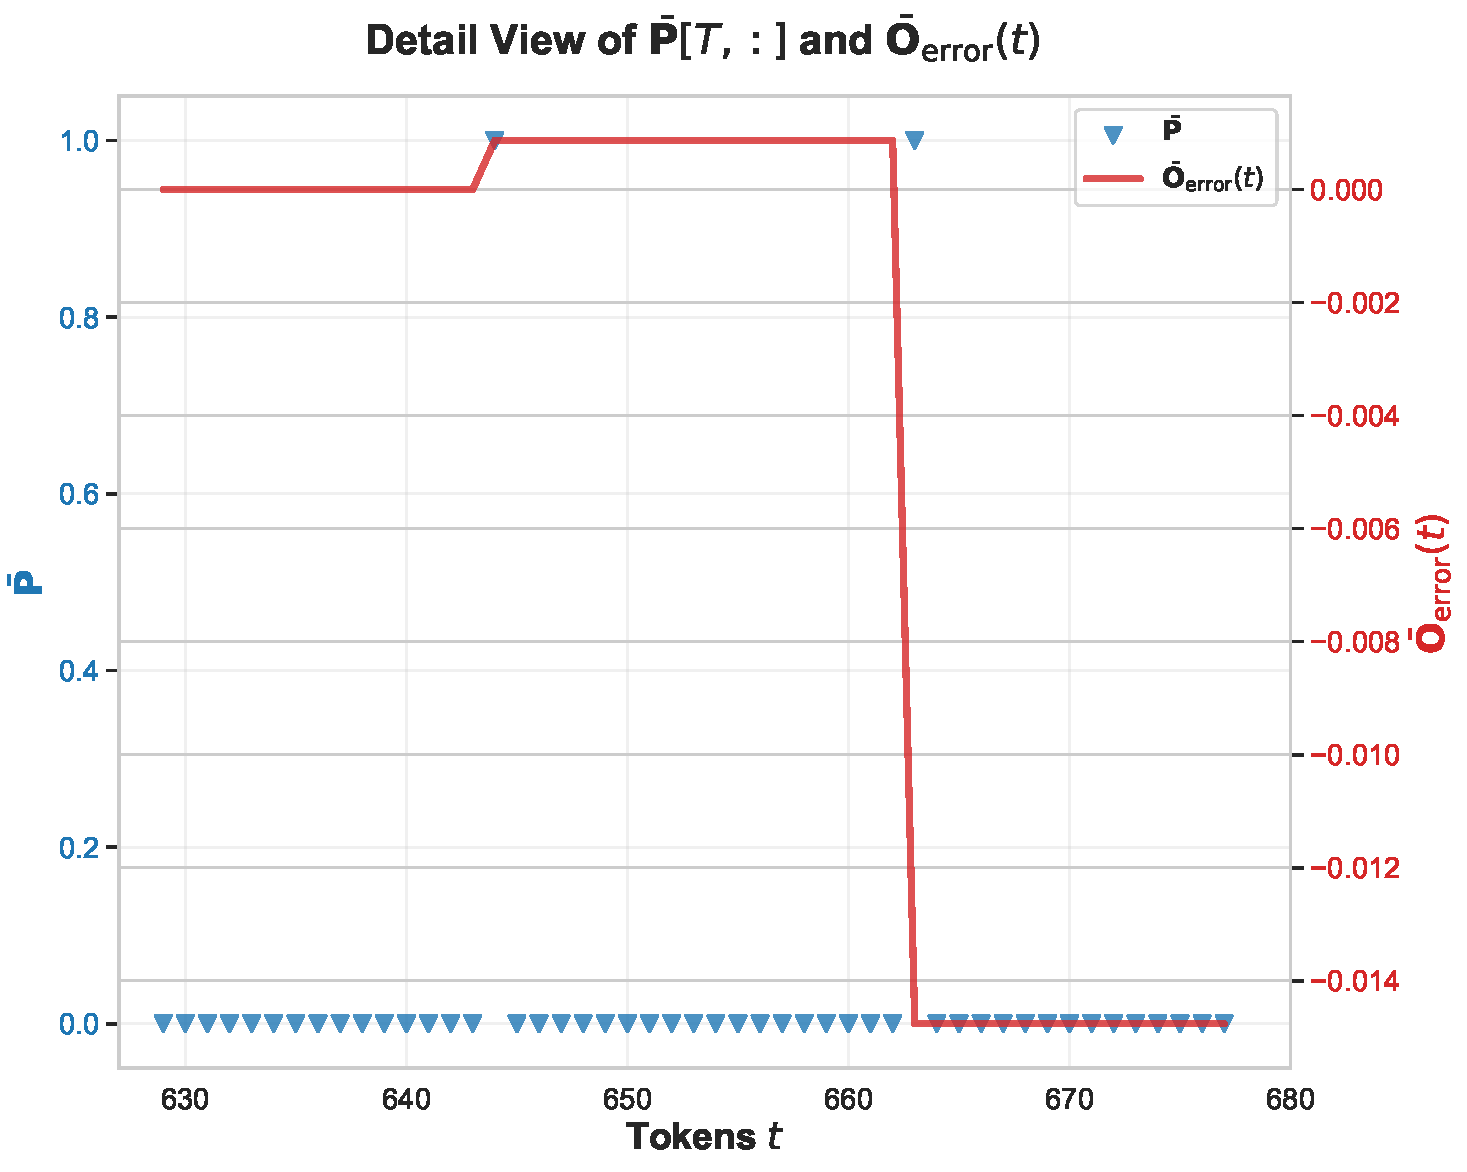
\includegraphics[width=0.32\textwidth]{img/detail_view_standalone.pdf}}
    \vspace{-10pt}
    \caption{分析 $\bar{\rmP}\rmV$}\label{fig:p_v_feature_analysis}
    % \vspace{-10px}
    % do_o_sample_analysis.ipynb
\end{figure}

\paragraph{找到 $(\rvdel_{lp} - \rvdel_{hp})[T]$} 中的大误差 我们首先调查 $\sum_{T=1}^N (\rvdel_{lp} - \rvdel_{hp})[T]$ 中正偏差的来源。正如 \cref{ssec:narrow} 中分析的那样，$\rvdel$ 中的误差源于上游梯度 $d\rmO$ 与低精度输出中的数值误差 $\rmO_{lp} - \rmO_{hp}$ 的乘积。为了剖析这一点，我们关注标记位置 $T=718$，其中误差分量 $(\rvdel_{lp} - \rvdel_{hp})[T]$ 是积极的。
% T = 718
% batch_id 854 -> 254
% training step 6619

在 \cref{fig:D_do_o_analysis}(b) 和 (c) 中，我们观察到梯度 $d\rmO[T, :]$ 与输出误差 $\rmO_{lp}[T, :] - \rmO_{hp}[T, :]$ 在特定特征维度（如 20 和 29，其他标记中亦有观察）上具有很强的符号相关性。在这些维度上，$d\rmO$ 与输出误差 $\rmO_{lp} - \rmO_{hp}$ 一直为负。这种对齐确保其乘积（导致 $\rvdel$ 的误差项）为正。事实上，输出误差往往为负（$\rmO_{lp}[T, i] < \rmO_{hp}[T, i]$），表明低精度计算 $\rmO$ 系统性地偏向更负的数值。因此，我们后续分析重点在于确定这种计算偏差的根源。

输出 $\rmO$ 根据中间非标准化输出计算得出， $\bar{\rmO}$。计算涉及安全 softmax，然后是矩阵乘法和归一化：
\begin{align*}
  \bar{\rmP} &= \exp(\rmS - \mathrm{rowmax}(\rmS)), & \bar{\rmO} &= \bar{\rmP}\rmV, & \rmO &= \bar{\rmO} / \mathrm{rowsum}(\bar{\rmP}).
\end{align*}
进一步的实验查明了非标准化输出计算失败的根源， $\bar{\rmO} = \bar{\rmP}\rmV$。我们发现仅在 FP32 中计算该乘积就足以稳定训练。为了理解这种偏差的根源，我们检查了单个元素的低精度和高精度计算之间的差异， $\bar{\rmO}[T, i]$ （对于特征索引 $i=20$ 在我们的分析中）：
\begin{equation}
  \bar{\rmO}_{lp}[T, i] - \bar{\rmO}_{hp}[T, i] = (\bar{\rmP}_{lp}[T, :]\rmV[:, i])_{lp} - (\bar{\rmP}_{hp}[T, :]\rmV[:, i])_{hp}
\end{equation}
其中输入 $\bar{\rmP}$ 和 $\rmV$ 本身就是先前 BF16 操作的结果。具体来说，下标 $(\cdot)_{lp}$ 这里计算 FP32 中的点积，最终结果四舍五入为 BF16，而 $(\cdot)_{hp}$ 完全用 FP32 计算。


要了解错误是如何发生的 $\bar{\rmO}_{lp}[T, i] - \bar{\rmO}_{hp}[T, i]$ 系统性地变为负值，我们绘制了随着代币头寸总和的进展而产生的累积误差 \cref{fig:p_v_feature_analysis}(b)和(c)：
\begin{equation}
\bar{\rmO}_{\text{error}}(t) 
= \left( \sum\nolimits_{t^\prime=1}^{t} \bar{\rmP}[T, t^\prime]\rmV[t^\prime, i] \right)_{lp} 
- \left( \sum\nolimits_{t^\prime=1}^{t} \bar{\rmP}[T, t^\prime]\rmV[t^\prime, i] \right)_{hp}.
\end{equation}
该图显示误差以显着的负步长累积。这些步骤发生在令牌位置 $t$ 其中相应的注意力概率 $\bar{\rmP}[T, t]$ 恰好为 1（在其他标记位置也观察到）。当 pre-softmax 得分时会发生这种情况 $\rmS[T, t]$ 是其行中的最大值，导致 $\exp(\rmS[T, t] - \max(\rmS[T, :]))$ 评估为 $\exp(0)=1$.

% \vspace{-10px}
\paragraph{偏差舍入误差分析}
此外，偏差是由这些单位值与值矩阵的分布的相互作用产生的 $\rmV$。正如观察到的 \cref{fig:p_v_feature_analysis}(a)，对于有问题的特征维度 $i=20$，值 $\rmV[:, i]$ 均以负面为主。什么时候 $\bar{\rmP}[T, t]=1$，产品 $\bar{\rmP}[T, t]\rmV[t, i]$ 简直就是 $\rmV[t, i]$，负 BF16 数。
\emph{当两个这样的负 BF16 数相加时会产生系统性误差。} 在浮点运算中，将两个同号数字相加可能会导致结果有效数溢出（例如， $\mathtt{-1.xxxx} + \mathtt{-1.yyyy}=\mathtt{-10.zzzz}$），从而需要右移并增加指数以重新归一化。被移出的 7 位 BF16 小数位决定舍入方向。当两个负数相加时，舍入操作（例如“舍入到最接近”）可能会引入一致性偏差。

为了说明这种舍入偏差是如何发生的，请考虑两个尾数相加会导致溢出，从而需要右移进行标准化。移出的位（舍入位）决定舍入方向。我们显示了最后两个 2 位数字的所有可能的加法，其中绿色位代表将被移出的位（舍入位）：
% \vspace{-5px}
\begin{tcolorbox}[colback=black!5!white,
  colframe=black,
  boxrule=0.5pt,
  width=0.95\linewidth,
  arc=4pt,
  boxsep=1pt,
  halign=center,
  top=0pt,
  bottom=0.5pt,
  center
]
\vspace{-5pt}
\begin{align*}
  \mathtt{00}+\mathtt{00}=\mathtt{0}&{\color{green}\mathtt{0}} &\; \mathtt{00} + \mathtt{01} = \mathtt{0}&{\color{green}\mathtt{1}}& \; \mathtt{00} + \mathtt{10} = \mathtt{1}&{\color{green}\mathtt{0}} &\; \mathtt{00} + \mathtt{11} = \mathtt{1}&{\color{green}\mathtt{1}} &\; \mathtt{01} + \mathtt{01} = \mathtt{1}&{\color{green}\mathtt{0}} \\
  \mathtt{01} + \mathtt{10} = \mathtt{1}&{\color{green}\mathtt{1}} &\; \mathtt{01} + \mathtt{11} = \mathtt{10}&{\color{green}\mathtt{0}}& \; \mathtt{10}+\mathtt{10}=\mathtt{10}&{\color{green}\mathtt{0}} &\; \mathtt{10} + \mathtt{11} = \mathtt{10}&{\color{green}\mathtt{1}} &\; \mathtt{11} + \mathtt{11} = \mathtt{11}&{\color{green}\mathtt{0}}
\end{align*}
\end{tcolorbox}
% \vspace{-5px}
由于求和是在 FP32 中执行的，因此小数字的低位累加可以激活粘滞位。因此，当添加后续 BF16 数字时，这会强制向上舍入。因此，舍入位 ${\color{green}\mathtt{1}}$ 表示需要向上舍入。因为操作数 $\bar{\rmP}[T, t]\rmV[t, i]$ 是负数并且有一个大指数（因为 $\bar{\rmP}[T, t]=1$ 不使 $\bar{\rmP}[T, t]\rmV[t, i]$ 较小），四舍五入的误差被放大，产生负误差。当舍入位为 ${\color{green}\mathtt{0}}$，结果向下舍入，引入正误差。
此外，与向上舍入产生的负误差相比，正误差更小，因为添加的值通常非常小。这种不对称导致舍入误差以向上舍入为主，从而导致我们的分析中观察到的负舍入误差。计算中的这种系统性负偏差 $\bar{\rmO}$ 是训练失败的最终根源。

\begin{remark}
  为了 $\bar{\rmP}[T, t] < 1$，其乘积为 $\rmV[t, i]$ 具有非零的至少 16 位。当舍入到 BF16 时，这不会引入有偏差的舍入误差。
\end{remark}

% \vspace{-20px}
\paragraph{\cref{fig:p_v_feature_analysis} 中的舍入误差分析}
为了具体说明这一点，我们现在分析导致大负误差跳跃的具体 BF16 数加法，如图所示 \cref{fig:p_v_feature_analysis}（三）。因为求和是在 FP32 中执行的，所以在添加第二个 BF16 值之前，第一个 BF16 值会加上其他令牌的一些小值。这可以激活粘性位，在添加第二个 BF16 值时可以强制向上舍入。
对于此示例，我们从 FP32 表示开始。
第一个操作数是前面各项的累加和，其中包括 BF16 ($\mathtt{1}{{\color{red}\mathtt{10000000}}}{{\color{blue}\mathtt{0011010}}}{\color{gray}\mathtt{0000000000000000}}; -2.40625$）加上小的残差（$\sim 0.00087$）激活粘滞位。第二个操作数是另一个 BF16 值。他们的 FP32 表示是：
% \vspace{-5px}
\begin{tcolorbox}[colback=black!5!white,
  colframe=black,
  boxrule=0.5pt,
  width=0.95\linewidth,
  arc=4pt,
  boxsep=1pt,
  halign=center,
  top=0pt,
  bottom=0.5pt,
  center]
\vspace{-5pt}
\begin{align*}
  \mathtt{1}{\color{red}\mathtt{10000000}}{\color{blue}\mathtt{0011010}}{\color{gray}\mathtt{0000111000101110}} &\; (-2.4071154594421387) \\
  \mathtt{1}{{\color{red}\mathtt{10000000}}}{{\color{blue}\mathtt{0010011}}}{\color{gray}\mathtt{0000000000000000}}&\; (-2.296875)
\end{align*}
\end{tcolorbox}
% \vspace{-5px}
由于它们的指数相同，因此对它们的有效数进行加法：
% \vspace{-5px}
\begin{tcolorbox}[colback=black!5!white,
  colframe=black,
  boxrule=0.5pt,
  width=0.95\linewidth,
  arc=4pt,
  boxsep=1pt,
  halign=center,
  top=0pt,
  bottom=0.5pt,
  center]
\vspace{-4pt}
\begin{align*}
  &(\mathtt{-1.}{\color{blue}\mathtt{0011010}}{\color{gray}\mathtt{0000111000101110}})
  + (\mathtt{-1.}{\color{blue}\mathtt{0010011}}{\color{gray}\mathtt{0000000000000000}})& \\
  =& -\mathtt{10.{\color{blue}0101101}}{\color{gray}\mathtt{0000111000101110}}
\end{align*}
\end{tcolorbox}
% \vspace{-5px}
结果溢出有效数字的格式，需要标准化。尾数右移一位，指数递增：
% \vspace{-5px}
\begin{tcolorbox}[colback=black!5!white,
  colframe=black,
  boxrule=0.5pt,
  width=0.95\linewidth,
  arc=4pt,
  boxsep=1pt,
  halign=center,
  top=0pt,
  bottom=0.5pt,
  center]
\vspace{-4pt}
\begin{align*}
  \text{Significand: } \mathtt{10.{\color{blue}0101101}} \to \mathtt{1.{\color{blue}0010110}{\color{green}1}} \quad \quad
  \text{Exponent: } {\color{red}\mathtt{10000000}} \to {\color{red}\mathtt{10000001}}
\end{align*}
\end{tcolorbox}
% \vspace{-5px}
FP32 中的确切结果是 $\mathtt{1}\,{\color{red}\mathtt{10000001}}\,{\color{blue}\mathtt{0010110}}{\color{green}\mathtt{1}}{\color{gray}\mathtt{000011100010111}}$，对应于 $-4.703990459442139$。要将此结果存储在 BF16 中，必须将其舍入为 7 个小数位。有效数是 $\mathtt{1.{\color{blue}0010110}{\color{green}1}}$。 7 位分数是 ${\color{blue}\mathtt{0010110}}$。因为舍入位是 ${\color{green}\mathtt{1}}$ 并且舍入位后有非零位，舍入到最接近的（偶数）规则向上舍入（将 1 添加到分数的最后一位）：
% \vspace{-5px}
\begin{tcolorbox}[colback=black!5!white,
  colframe=black,
  boxrule=0.5pt,
  width=0.95\linewidth,
  arc=4pt,
  boxsep=1pt,
  halign=center,
  top=0pt,
  bottom=0.5pt,
  center]
\vspace{-4pt}
  \begin{align*}
  \text{BF16 Fraction: } {\color{blue}\mathtt{0010110}} + \mathtt{1} = {\color{blue}\mathtt{0010111}}
\end{align*}
\end{tcolorbox}
% \vspace{-5px}
BF16最终结果是 $\mathtt{1}{\color{red}\mathtt{10000001}}{\color{blue}\mathtt{0010111}}$，这代表 $-4.71875$。这个四舍五入的值比真实的总和更负 $-4.703990459442139$。这个单一添加引入的错误是 $\mathbf{-0.014759540557861328}$。当这种舍入事件在许多添加中系统地发生时 $\bar{\rmP}\rmV$ 产品中，错误会累积，从而产生负面偏差 $\rmO$ 最终破坏训练的稳定性。



% \vspace{-5px}
\begin{tcolorbox}[
  colback=cyan!5!white,
  colframe=black!100,
  boxrule=0.4pt,
  arc=3pt,
  left=5pt, right=5pt,
  top=5pt, bottom=5pt,
  width=0.95\linewidth,
  coltitle=black,
  center
]
\begin{claim}\label{claim3}
  与不止一个 $\bar{\rmP}[T,t]=1$ 和消极的 $\rmV[t, i]$，添加在 $\bar{\rmP}\rmV$ 可能会导致有效数溢出。由于粘性位，这需要右移和有效数字舍入，从而在 $\rmO$ 并导致积极的 $(\rvdel_{lp} - \rvdel_{hp})[T]$.
\end{claim}
\end{tcolorbox}




% \vspace{-10px}
\section{实验：减轻舍入误差中的偏差}\label{sec:stable_fa}


我们的分析追踪了偏差舍入误差的失败 $\bar{\rmP}\rmV$ 计算。当 pre-softmax 分数的一行中有多个相同的最大值时，就会发生这种情况 $\rmS$ 导致相应的元素 $\bar{\rmP}$ 正好变成 1。为了验证我们的发现，我们修改了 softmax 来检测这个特定条件并调整归一化，确保 $\bar{\rmP}$ 严格小于 1。这可以防止有偏差的舍入并恢复训练稳定性。

\begin{wrapfigure}{r}{0.5\textwidth}
%\vspace{-20px}
\begin{align*}
\rvr_m &= \mathrm{rowmax}(\rmS), \quad \rvr_s = \mathrm{rowsum}(\rmS \equiv \rvr_m) \\
\rvm^\prime &= \mathrm{where}(\rvr_m > 0 \land \rvr_s > 1, \beta \rvr_m, \rvr_m), \beta > 1 \\
\rvm &= \mathrm{where}(\rvr_m < 0 \land \rvr_s > 1, 0, \rvm^\prime) \\
\bar{\rmP} &= \exp(\rmS - \rvm)
\end{align*}
\vspace{-25pt}
\end{wrapfigure}
为了防止舍入偏差，我们对安全 softmax 计算进行了有针对性的修改。核心思想是动态调整归一化因子 $\rvm$ 仅当分数矩阵的一行 $\rmS$ 包含多个相同的最大值。这种调整确保指数函数的参数， $\rmS - \rvm$，在这些最大位置处变为严格负数，这反过来又保证了 $\bar{\rmP} = \exp(\rmS - \rvm)$ 小于 1。简单的方法（例如减去一个小的固定常数）是不够的，因为它引入了新的系统舍入误差（请参阅 \cref{app:design_consider}）；因此，需要动态最大化策略。我们的修改如上所示。

\begin{wrapfigure}{r}{0.4\textwidth}
	\centering
	% \vspace{-20px}
	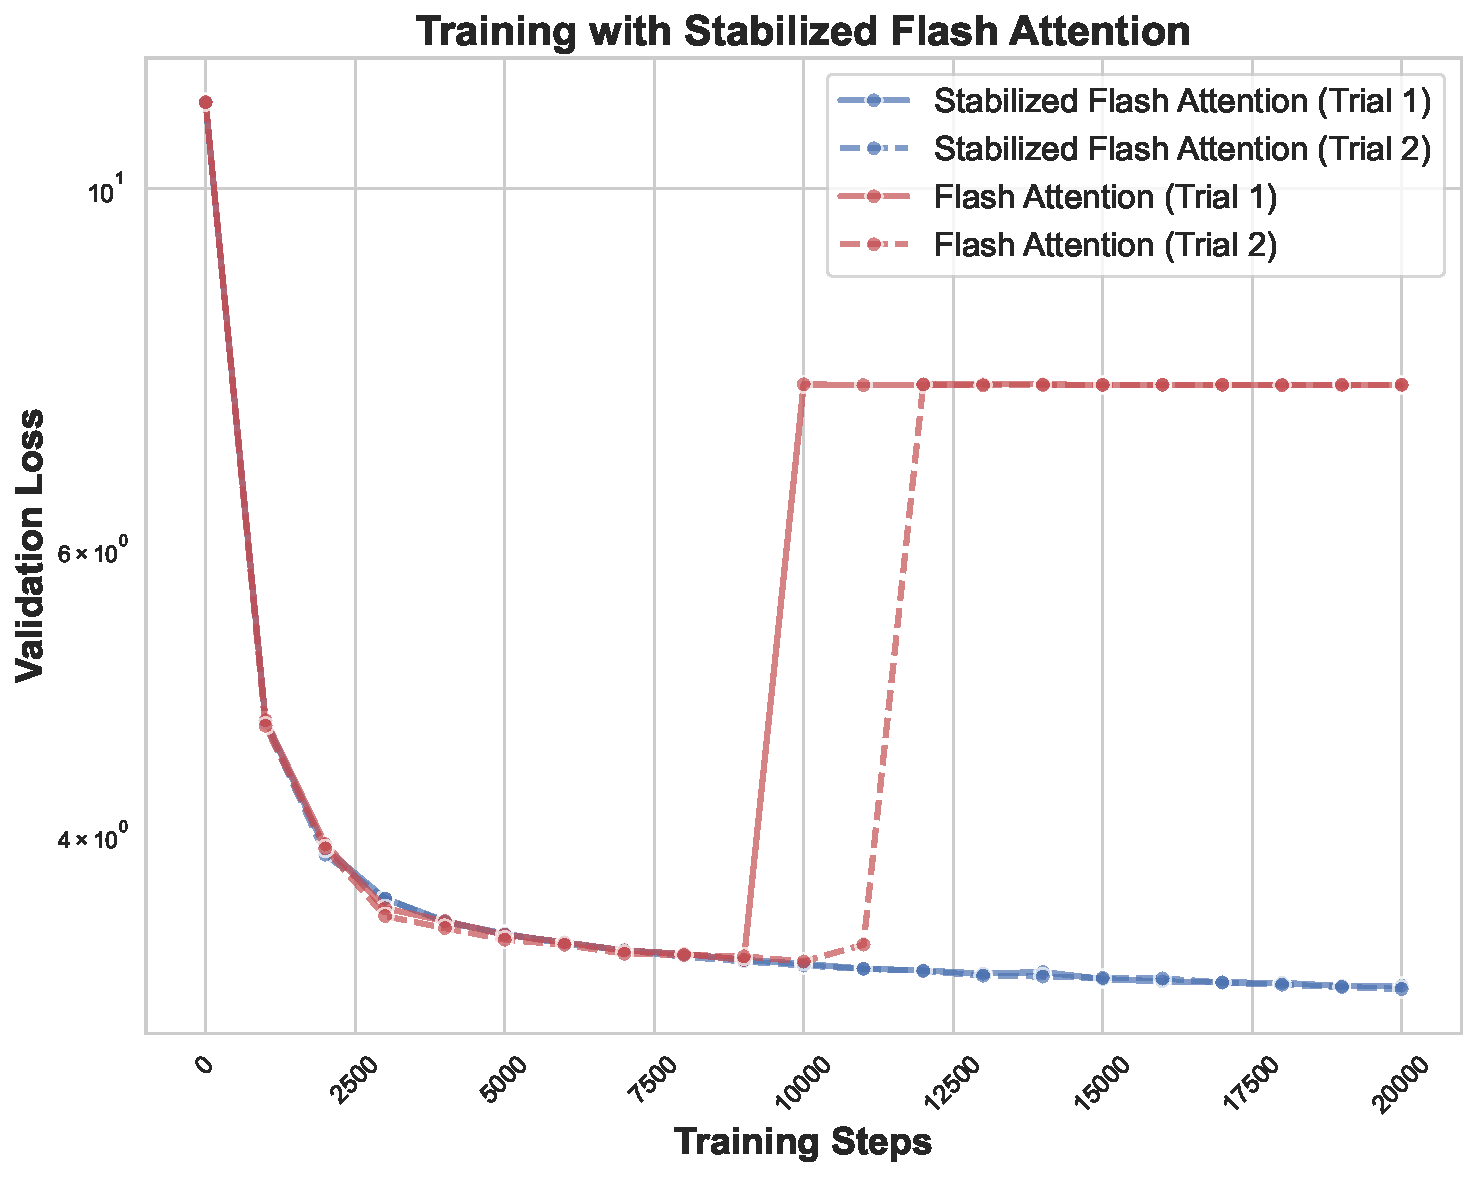
\includegraphics[width=0.4\textwidth]{img/SFA_FA_loss.pdf}
	% \vspace{-20px}
  \caption{稳定化 FA 与原始 FA 的对比。}\label{fig:stable_fa_comparison}
	% \vspace{-20px}
	% visualize_SFA_loss.py
\end{wrapfigure}


此修改可防止以下元素 $\bar{\rmP}$ 从正好 1 开始。如果一行的最大值， $\rvr_m$，为正且重复，归一化因子调整为 $\rvm = \beta \rvr_m$ （和 $\beta > 1$）。这使得指数达到新的最大值 $-(\beta - 1)\rvr_m$，严格来说是负数。如果 $\rvr_m$ 为负数且重复，我们设 $\rvm = 0$，这也确保指数的最大值保持为负数。在这两种情况下，此调整都保证 $\max(\rmS - \rvm) < 0$ 因此 $\max(\bar{\rmP}) < 1$，防止导致有偏差舍入的情况。



至关重要的是，这种修改在数学上等价于精确算术中的标准注意力，因为它利用了 softmax 函数的平移不变性（$\mathrm{softmax}(\mathbf{z}) = \mathrm{softmax}(\mathbf{z} - c)$）。我们的方法只是选择不同的行常量 $c$ 以确保数值稳定性。在我们的实验中，我们设置 $\beta \in [2, 8]$，因为较小的值有将结果舍入为 1 的风险，而较大的值则有下溢的风险。此修改已集成到标准 Flash Attention 平铺算法中（如 \cref{alg:SFA} 中的{\color{magenta}洋红色}行所示），且不改变反向过程。如图所示 \cref{fig:stable_fa_comparison}，这个简单的改变（$\beta=7$）成功稳定了训练，证实了我们的分析。进一步的设计细节见 \cref{app:design_consider}。



\section{结论}

本文对低精度 Flash Attention 训练中臭名昭著的损失爆炸提出了第一个机制性解释。我们查明了新出现的低秩表示和有偏的 BF16 舍入误差之间相互作用的根本原因。对 Flash Attention 进行最小化且有针对性的修改可以通过恢复稳定性来验证我们的分析。我们的分析工作流程为诊断其他架构、尺度和低精度格式中的类似数值不稳定性提供了蓝图，为更稳健、更高效的大规模模型训练铺平了道路。

\paragraph{讨论}
我们的研究结果在各种硬件（NVIDIA A100、RTX 4090、华为 Ascend 910B）中都是一致的，并从机制上解释了训练不稳定的经验观察结果。权重谱范数的增长是梯度中低秩误差矩阵累积的结果。我们还阐明了注意力池的作用：通过吸引高注意力分数，它们更有可能产生 1 的注意力概率，这会触发 $\bar{\rmP}\rmV$ 计算。这在接收器的架构行为和导致训练脱轨的算术不稳定性之间提供了直接的数值联系。

\paragraph{局限性}
我们的分析重点是 GPT-2 模型中的特定失败案例。我们的研究结果是否适用于其他架构、更大的尺度或不同的低精度格式（如 FP8）需要进一步研究。此外，我们提出的缓解措施是针对所识别的特定舍入误差量身定制的，可能无法解决其他数值不稳定来源。


% \subsubsection*{Author Contributions}
% If you'd like to, you may include  a section for author contributions as is done
% in many journals. This is optional and at the discretion of the authors.

% \subsubsection*{Acknowledgments}
% Use unnumbered third level headings for the acknowledgments. All
% acknowledgments, including those to funding agencies, go at the end of the paper.

\nocite{*} % 这将包括参考书目中的所有参考文献，即使文本中没有引用。
\bibliography{iclr2026_conference}
\bibliographystyle{iclr2026_conference}

\newpage
\appendix


\section{相关工作}


\subsection{混合精度 BF16 训练。}  
当代大语言模型（LLM）预训练几乎普遍采用混合精度算术。早期的努力 \citet{micikevicius2017mixed} 证明 FP16 训练（使用权重的 FP32 主副本和固定损失缩放）可以与许多模型的 FP32 准确性相匹配。然而，FP16 的指数范围较窄，通常会导致许多梯度下溢，因此需要仔细调整。 bfloat16 (BF16) 格式具有 8 位指数和 7 位尾数，保留了 FP32 的宽动态范围，同时将存储成本减半。 \citet{kalamkar2019study} 表明 BF16 在大型模型上无需专门调整即可实现与 FP32 的收敛同等性。自此，BF16成为很多大型训练框架默认的16位格式，并在PyTorch和TensorFlow中原生支持~\citep{wang2019bfloat16}. 

BF16 混合精度使具有里程碑意义的 LLM 能够以前所未有的规模进行训练，包括 GPT-3 (175B) \citep{brown2020language}, 谷歌PaLM (540B) \citep{chowdhery2023palm}、DeepMind Gopher (280B) \citep{rae2021scaling}, 龙猫(70B) \citep{hoffmann2022training}，以及 Meta 的 LLaMA 系列 (7B-65B) \citep{touvron2023llama}。为了处理大量内存占用，Megatron 和 DeepSpeed 等并行训练框架将 BF16 训练与零冗余优化器 (ZeRO) 等技术集成 \citep{rajbhandari2020zero}.

尽管有其优点，BF16 训练仍然会表现出不稳定性。实证研究表明，即使在损失缩放的情况下，FP16 也高度不稳定，而 BF16 消除了大多数与精度相关的调整和故障 \cite{wang2019bfloat16}。然而， \citet{lee2024fp8} 报告称，在纯 BF16 下，大约 10\% 的 GPT-2 预训练运行出现了偏差，而在 TF32 下，这一比例为 0\%。这表明，虽然 BF16 显着提高了稳定性，但大规模的补充稳定技术仍然是必要的。 

\subsection{稳定低精度训练}

\paragraph{梯度缩放。}
早期作品由 \citet{micikevicius2017mixed} 引入了 FP16 混合精度训练，其中权重、激活和梯度以半精度存储，同时维护主 FP32 副本。他们还提出 \textit{loss scaling} 以防止 FP16 下溢。即使有损失缩放，深度网络中仍然可能发生一些下溢。为了解决这个问题， \citet{zhao2021reducing} 介绍 \textit{gradient scaling}，它动态计算每层缩放因子以避免下溢和溢出。

\paragraph{超低精度 (FP8/INT8) 训练。}
为了进一步降低成本，最近的工作探索了用于训练和推理的 FP8 或 INT8 精度。
然而，简单的 FP8 训练往往会出现分歧。 \citet{lee2024fp8} 请注意，如果没有额外的稳定技术，直接将 FP8 应用于 LLM 训练是不稳定的。
为了解决这个问题， \citet{perez2023training} 为 FP8 矩阵乘法提出动态调整的每张量缩放因子。 
使用该方案，他们完全在 FP8 中成功训练了高达 70B 参数的 GPT 和 LLaMA 型模型。
相似地， \citet{peng2023fp8} 介绍 \textsc{FP8-LM}，一个逐步将 FP8 应用于梯度、优化器状态和分布式通信的框架，与 BF16 相比，实现了 39% 的内存减少和 75% 的加速。
\citet{balancca2024scalify} 展示 \textsc{Scalify}，它在整个计算图中传播比例因子，以确保 FP8 稳定运行，无需手动调整。
这些方法共同证明，仔细的扩展管理使 FP8 或 INT8 训练能够匹配 BF16 性能，同时减少内存和计算需求。

\paragraph{优化器和梯度稳定。}
优化器算法在训练稳定性中起着至关重要的作用。
\citet{molybog2023theory} 从理论上分析 Adam 并表明，当大规模模型中更新方向与真实下降方向不相关时，通常会出现灾难性发散。
为了解决梯度不稳定问题， \citet{huang2025spam} 提出 \textsc{SPAM} （带动量重置的尖峰感知亚当），它通过重置动量和应用尖峰感知剪裁来检测和减轻罕见但严重的“梯度尖峰”。 
并联， \citet{wortsman2023stable} 研究视觉语言模型中的损失峰值，结果表明 AdamW 经常低估峰值发生前的第二个时刻。 
他们提出了一种混合 AdamW-AdaFactor 优化器，可以自适应地纠正二阶矩低估，优于单独的梯度裁剪。
这些方法强调了优化器修改如何直接减轻低精度状态下的发散。

\paragraph{激活和架构技术。}
激活函数和初始化策略的选择也会影响稳定性。
\citet{fishman2024scaling} 观察到 SwiGLU 激活在长时间 FP8 训练运行期间放大了异常值。他们介绍 \textit{Smooth-SwiGLU}，一种经过修改的激活，可防止异常值放大，从而实现稳定的万亿代币 FP8 训练。
在视觉语言领域， \citet{wortsman2023stable} 表明“层规模零”初始化和精心设计的低精度线性层（例如 SwitchBack）进一步提高了 int8 训练的稳定性。



\section{BF16 加法}\label{app:bf16_add}

bfloat16（大脑浮点）格式是一种 16 位浮点表示形式，因其计算效率和数值范围之间的平衡而广泛应用于深度学习。它由 1 个符号位、8 个指数位和 7 个小数（或尾数）位组成。此结构为 bfloat16 提供了与 32 位单精度格式 (FP32) 相同的动态范围，但精度明显较低。

两个 bfloat16 数字相加，例如 $a$ 和 $b$，遵循浮点运算的标准过程：
\begin{enumerate}[leftmargin=*]
    \item \textbf{Exponent Alignment:} 比较两个数字的指数。指数较小的数字的尾数（隐式前导位和小数的组合）向右移动，直到其指数与较大的指数匹配。每右移一次，指数就会增加一。移位超过可用精度的位将会丢失，这是错误的最初来源。
    \item \textbf{Significand Addition:} 对齐的有效数相加。结果的符号由操作数的符号和大小决定。
    \item \textbf{Normalization:} 结果被归一化以确保其符合 $\mathtt{1.xxxx...} \times 2^{e}$ 格式。如果添加导致溢出（例如， $\mathtt{10.xxxx...}$)，尾数右移，指数递增。如果它导致取消（例如， $\mathtt{0.00xx...}$)，尾数左移，指数递减，直到前导位为 $\mathtt{1}$.
    \item \textbf{Rounding:} 所得到的有效数在归一化后可能具有超过 7 个小数位，因此必须进行舍入。标准模式是“舍入到最接近，联系到偶数”。这意味着如果截断的部分大于最后可存储位 (LSB) 值的一半，则该数字将向上舍入。如果小于，则向下舍入。如果正好是一半，则四舍五入到最接近的具有偶数 LSB 的值。
\end{enumerate}

数值误差的关键来源来自步骤 1 和 4。在指数对齐期间，较小数值的数字会导致精度丢失。加法之后，结果必须四舍五入回到 7 位小数，这会引入另一个舍入误差。虽然“舍入到最接近，联系到偶数”被设计为对随机数据无偏，但对具有特定分布的数据进行一系列相加（例如，大多数负数相加在一起）可能会导致 \emph{biased rounding error}，其中累积误差始终将结果推向一个方向。这种偏差误差的积累是在低精度设置中观察到的训练失败的关键因素。


\section{减轻 Flash Attention 中的偏差舍入误差的设计注意事项}\label{app:design_consider}

\paragraph{使用动态最大值而不是固定偏移} 固定偏移会导致 \ensuremath{\bar{\rmP}} 的计算值在 BF16 转换期间在一个方向上一致舍入，从而引入固定误差。由于 \ensuremath{\rmV} 的元素通常具有相同的符号，因此 \ensuremath{\bar{\rmP}} 中的固定舍入误差在计算 \ensuremath{\bar{\rmP}\rmV} 时不会平均为零。这会在输出 \ensuremath{\rmO} 中产生有偏误差，进而形成有偏的 \ensuremath{\rvdel} 项，重新引入我们旨在解决的失败。


\paragraph{有条件地应用动态最大值} 我们的修改是有条件地应用的——仅当一行包含多个相同的最大值时——以避免引入新的数值不稳定性。无条件调整并不是更好的选择。例如，如果一行有一个非常大的正最大值 $\rvr_m$，应用我们的规则意味着计算 $\exp(\rmS - \beta\rvr_m)$。指数中最大的项将变为 $-(\beta-1)\rvr_m$， 和 $\exp(-(\beta-1)\rvr_m)$ 可能下溢至零。这将导致归一化因子变为零，从而在计算输出时导致除零错误 $\rmO$。通过仅在导致有偏差舍入的特定情况下应用修改，我们在所有其他情况下保持了标准在线 softmax 的数值稳定性。


\paragraph{负重复行最大值处理说明} 我们还探索了负的重复行最大值的替代稳定方法（$\rvr_m < 0$）。一种方法涉及设置标准化因子 $\rvm = \gamma \rvr_m$ 对于某些人来说 $\gamma \in (0, 1)$。这使得指数中的新最大值 $(1-\gamma) \rvr_m$。然而，我们观察到，如果 $\gamma$ 接近 1，这个新的最大值接近于零。在低精度算术中， $\exp((1-\gamma) \rvr_m)$ 可以精确地舍入为 1，从而重新引入我们旨在防止的失败。因此，我们发现设置 $\gamma=0$ (i.e., $\rvm=0$) 是一个稳健的选择，因为它确保指数中的最大值保持足够的负值。


\begin{algorithm}[h!]
  % \algsetup{linenosize=\tiny}
  \caption{通过缓解有偏舍入误差的稳定化 Flash Attention：前向过程}\label{alg:SFA}
  \begin{algorithmic}[1]
    \REQUIRE 矩阵 $\rmQ, \rmK, \rmV \in \mathbb{R}^{N \times d}$, 块大小 $B_c$, $B_r$, $\beta>1$.
    \STATE 划分 $\rmQ$ 进入 $T_r = \left\lceil\frac{N}{B_r} \right\rceil$ 块 $\rmQ_1, \dots, \rmQ_{T_r}$ 尺寸的 $B_r \times d$ 每个，
    并划分 $\rmK, \rmV$ in to $T_c = \left\lceil \frac{N}{B_c} \right\rceil$ 块 $\rmK_1, \dots, \rmK_{T_c}$ 和
    $\rmV_1, \dots, \rmV_{T_c}$，尺寸 $B_c \times d$ 每个。
    \STATE 划分输出 $\rmO \in \mathbb{R}^{N \times d}$ 进入 $T_r$ 块 $\rmO_1, \dots, \rmO_{T_r}$ 尺寸的
    $B_r \times d$ 每个，然后除logsumexp $\rmL$ 进入 $T_r$ 块 $\rmL_1, \dots, \rmL_{T_r}$ 尺寸的
    $B_r$ 每个。
    \FOR{$1 \le i \le T_r$}
      % \STATE Load $\rmQ_i$ from HBM to on-chip SRAM.
      \STATE 初始化 $\rmO_{i}^{(0)} = (0)_{B_r \times d} \in \mathbb{R}^{B_r \times d}, \rvell_{i}^{(0)} = (0)_{B_r} \in \mathbb{R}^{B_r}, \rvm_{i}^{(0)} = (-\infty)_{B_r} \in \mathbb{R}^{B_r}$.
      \FOR{$1 \le j \le T_c$}
        % \STATE Load $\rmK_j, \rmV_j$ from HBM to on-chip SRAM.
        \STATE 计算 $\rmS_{i}^{(j)} = \rmQ_i \rmK_j^T \in \mathbb{R}^{B_r \times B_c}$.
          \STATE {\color{magenta}$\rvr_m =  \mathrm{rowmax}(\rmS_{i}^{(j)})$, $\rvr_s = \mathrm{rowsum}(\rmS_{i}^{(j)} \equiv \rvr_m)$}
          \STATE {\color{magenta}$\rvm_{i}^{(j)\prime} = \mathrm{where}(\rvr_m > 0 \land \rvr_s > 1, \beta \rvr_m, \rvr_m)$}
          \STATE {\color{magenta}$\rvm_{i}^{(j)} = \mathrm{where}(\rvr_m < 0 \land \rvr_s > 1, 0, \rvm_{i}^{(j)\prime})$}
        \STATE 计算
        $\rvm_{i}^{(j)} = \mathrm{max}(\rvm_{i}^{(j-1)}, \rvr_m) \in \mathbb{R}^{B_r}$, $\bar{\rmP}_{i}^{(j)} = \exp(\rmS_{i}^{(j)} - \rvm_{i}^{(j)}) \in \mathbb{R}^{B_r \times B_c}$ （逐点），
        $\rvell_{i}^{(j)} = e^{\rvm_{i}^{(j-1)} - \rvm_{i}^{(j)}} \rvell_{i}^{(j-1)} + \mathrm{row sum}(\bar{\rmP}_{i}^{(j)}) \in \mathbb{R}^{B_r}$.
        \STATE 计算
        $\rmO_{i}^{(j)} = \text{diag}(e^{\rvm_{i}^{(j-1)} - \rvm_{i}^{(j)}}) \rmO_{i}^{(j-1)} + \bar{\rmP}_{i}^{(j)} \rmV_j$.
      \ENDFOR
      \STATE 计算 $\rmO_{i} = \text{diag}(\rvell_{i}^{(T_c)})^{-1} \rmO_{i}^{(T_c)}$.
      \STATE 计算 $\rmL_{i} = \rvm_{i}^{(T_c)} + \log(\rvell_{i}^{(T_c)})$.
      \STATE 写 $\rmO_{i}$ 作为 $i$第 块 $\rmO$.
      \STATE 写 $\rmL_{i}$ 作为 $i$第 块 $\rmL$.
    \ENDFOR
    \STATE 返回输出 $\rmO$ 和 logsumexp $\rmL$.
  \end{algorithmic}
\end{algorithm}


\begin{algorithm}[h!]
  % \algsetup{linenosize=\tiny}
  \caption{Flash Attention：前向过程}\label{alg:fa_forward}
  \begin{algorithmic}[1]
    \REQUIRE 矩阵 $\rmQ, \rmK, \rmV \in \mathbb{R}^{N \times d}$, 块大小 $B_c$, $B_r$.
    \STATE \label{alg:stream_attn_split_qkv} 划分 $\rmQ$ 进入 $T_r = \left\lceil\frac{N}{B_r} \right\rceil$ 块 $\rmQ_1, \dots, \rmQ_{T_r}$ 尺寸的 $B_r \times d$ 每个，
    并划分 $\rmK, \rmV$ in to $T_c = \left\lceil \frac{N}{B_c} \right\rceil$ 块 $\rmK_1, \dots, \rmK_{T_c}$ 和
    $\rmV_1, \dots, \rmV_{T_c}$，尺寸 $B_c \times d$ 每个。
    \STATE 划分输出 $\rmO \in \mathbb{R}^{N \times d}$ 进入 $T_r$ 块 $\rmO_1, \dots, \rmO_{T_r}$ 尺寸的
    $B_r \times d$ 每个，然后除logsumexp $\rmL$ 进入 $T_r$ 块 $\rmL_1, \dots, \rmL_{T_r}$ 尺寸的
    $B_r$ 每个。
    \FOR{$1 \le i \le T_r$} \label{alg:stream_attn_outer_loop}
      % \STATE \label{alg:stream_attn_load_q} Load $\rmQ_i$ from HBM to on-chip SRAM.
      \STATE 初始化 $\rmO_{i}^{(0)} = (0)_{B_r \times d} \in \mathbb{R}^{B_r \times d}, \rvell_{i}^{(0)} = (0)_{B_r} \in \mathbb{R}^{B_r}, \rvm_{i}^{(0)} = (-\infty)_{B_r} \in \mathbb{R}^{B_r}$.
      \FOR{$1 \le j \le T_c$}
        % \STATE \label{alg:stream_attn_load_kv} Load $\rmK_j, \rmV_j$ from HBM to on-chip SRAM.
        \STATE 计算 $\rmS_{i}^{(j)} = \rmQ_i \rmK_j^T \in \mathbb{R}^{B_r \times B_c}$.
        \STATE 计算
        $\rvm_{i}^{(j)} = \mathrm{max}(\rvm_{i}^{(j-1)}, \mathrm{rowmax}(\rmS_{i}^{(j)})) \in \mathbb{R}^{B_r}$, $\bar{\rmP}_{i}^{(j)} = \exp(\rmS_{i}^{(j)} - \rvm_{i}^{(j)}) \in \mathbb{R}^{B_r \times B_c}$ （逐点），
        $\rvell_{i}^{(j)} = e^{\rvm_{i}^{(j-1)} - \rvm_{i}^{(j)}} \rvell_{i}^{(j-1)} + \mathrm{row sum}(\bar{\rmP}_{i}^{(j)}) \in \mathbb{R}^{B_r}$.
        \STATE 计算
        $\rmO_{i}^{(j)} = \text{diag}(e^{\rvm_{i}^{(j-1)} - \rvm_{i}^{(j)}}) \rmO_{i}^{(j-1)} + \bar{\rmP}_{i}^{(j)} \rmV_j$.
      \ENDFOR
      \STATE 计算 $\rmO_{i} = \text{diag}(\rvell_{i}^{(T_c)})^{-1} \rmO_{i}^{(T_c)}$.
      \STATE 计算 $\rmL_{i} = \rvm_{i}^{(T_c)} + \log(\rvell_{i}^{(T_c)})$.
      \STATE 写 $\rmO_{i}$ 作为 $i$第 块 $\rmO$.
      \STATE 写 $\rmL_{i}$ 作为 $i$第 块 $\rmL$.
    \ENDFOR
    \STATE 返回输出 $\rmO$ 和 logsumexp $L$.
  \end{algorithmic}
\end{algorithm}

\begin{algorithm}[t]
  \caption{Flash Attention：反向过程}\label{alg:fa_backward}
  \begin{algorithmic}[1]
    \REQUIRE 矩阵 $\rmQ, \rmK, \rmV, \rmO, d\rmO \in \mathbb{R}^{N \times d}$,
    向量 $L \in \mathbb{R}^N$, 块大小 $B_c$, $B_r$.
    \STATE 划分 $\rmQ$ 进入 $T_r = \left\lceil\frac{N}{B_r} \right\rceil$ 块 $\rmQ_1, \dots, \rmQ_{T_r}$ 尺寸的 $B_r \times d$ 每个，
    并划分 $\rmK, \rmV$ in to $T_c = \left\lceil \frac{N}{B_c} \right\rceil$ 块 $\rmK_1, \dots, \rmK_{T_c}$ 和
    $\rmV_1, \dots, \rmV_{T_c}$，尺寸 $B_c \times d$ 每个。
    \STATE 划分 $\rmO$ 进入 $T_r$ 块 $\rmO_1, \dots, \rmO_{T_r}$ 尺寸的
    $B_r \times d$ 各，分 $d\rmO$ 进入 $T_r$ 块 $d\rmO_1, \dots, d\rmO_{T_r}$
    尺寸的 $B_r \times d$ 每个，并划分 $\rmL$ 进入 $T_r$ 块 $\rmL_1, \dots, \rmL_{T_r}$ 尺寸的
    $B_r$ 每个。
    \STATE 初始化 $d\rmQ = (0)_{N \times d}$ 并将其分为 $T_r$ 块 $d\rmQ_1, \dots, d\rmQ_{T_r}$ 尺寸的 $B_r \times d$ 每个。
    划分 $d\rmK, d\rmV \in \mathbb{R}^{N \times d}$ in to $T_c$ 块 $d\rmK_1, \dots, d\rmK_{T_c}$ 和
    $d\rmV_1, \dots, d\rmV_{T_c}$，尺寸 $B_c \times d$ 每个。
    \STATE 计算 $\rvdel = \mathrm{rowsum}(d\rmO \circ \rmO) \in \mathbb{R}^N$ （逐点相乘），然后将其分为 $T_r$ 块 $\rvdel_1, \dots, \rvdel_{T_r}$ 尺寸的
    $B_r$ 每个。
    \FOR{$1 \le j \le T_c$}
      % \STATE Load $\rmK_j, \rmV_j$ from HBM to on-chip SRAM.
      \STATE 初始化 $d\rmK_j = (0)_{B_c \times d}, d\rmV_j = (0)_{B_c \times d}$.
      \FOR{$1 \le i \le T_r$}
        % \STATE Load $\rmQ_i, \rmO_i, d\rmO_i, d\rmQ_i, L_i, \rvdel_i$ from HBM to on-chip SRAM.
        \STATE 计算 $\rmS_{i}^{(j)} = \rmQ_i \rmK_j^T \in \mathbb{R}^{B_r \times B_c}$.
        \STATE 计算 $\rmP_{i}^{(j)} = \exp(\rmS_{ij} - \rmL_{i}) \in \mathbb{R}^{B_r \times B_c}$.
        \STATE 计算
        $d\rmV_j \leftarrow d\rmV_j + (\rmP_{i}^{(j)})^\top d\rmO_i \in \mathbb{R}^{B_c \times d}$.
        \STATE 计算
        $d\rmP_{i}^{(j)} = d\rmO_{i} \rmV_j^\top \in \mathbb{R}^{B_r \times B_c}$.
        \STATE 计算 $d\rmS_{i}^{(j)} = \rmP_{i}^{(j)} \circ (d\rmP_{i}^{(j)} - \rvdel_i) \in \mathbb{R}^{B_r \times B_c}$.
        % \STATE Load $d\rmQ_i$ from HBM to SRAM, then on chip, update
        \STATE 更新 $d\rmQ_{i} \leftarrow d\rmQ_i + d\rmS_{i}^{(j)} \rmK_j \in \mathbb{R}^{B_r \times d}$.
        % , and write
        % back to HBM.
        \STATE 计算 $d\rmK_{j} \leftarrow d\rmK_j + {d\rmS_{i}^{(j)}}^\top d\rmQ_i \in \mathbb{R}^{B_c \times d}$.
      \ENDFOR
      % \STATE Write $d\rmK_j, d\rmV_j$ to HBM.
    \ENDFOR
    \STATE 返回 $d\rmQ, d\rmK, d\rmV$.
  \end{algorithmic}
\end{algorithm}

\begin{figure}[t]
\subfigure[nanoGPT Issue \#303 的损失曲线]{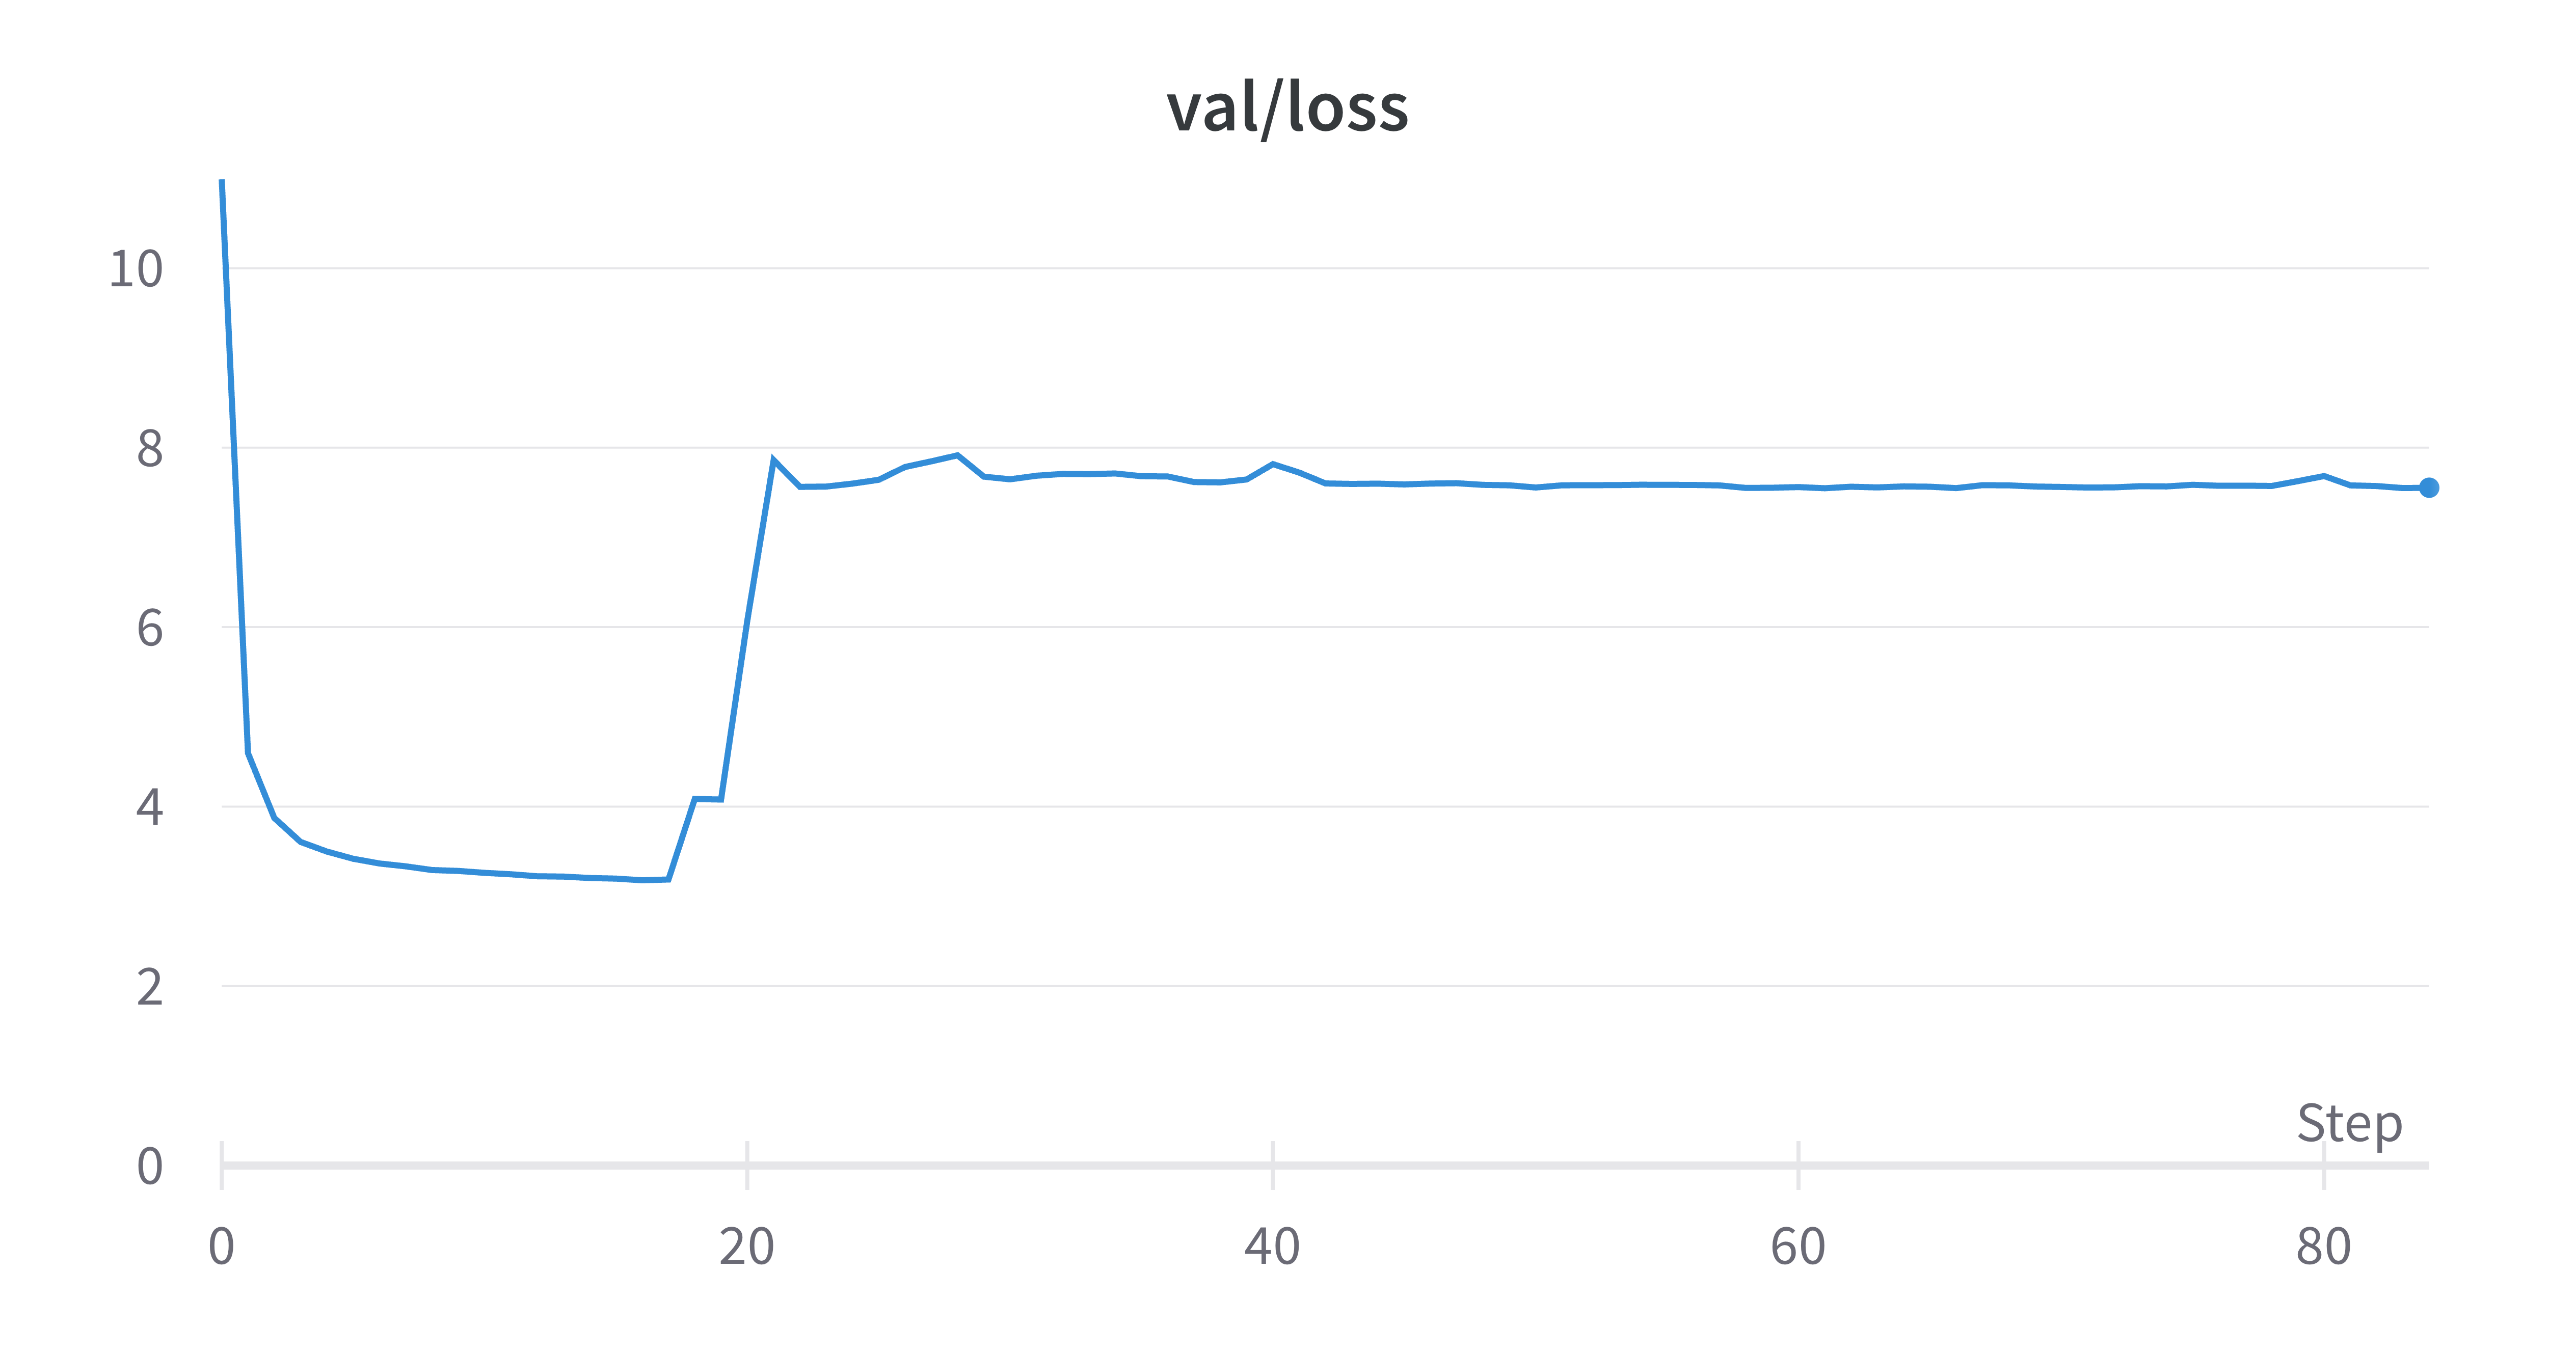
\includegraphics[width=\textwidth]{img/loss_in_nanogpt_303.png}  }
\subfigure[nanoGPT Issue \#524 的损失曲线]{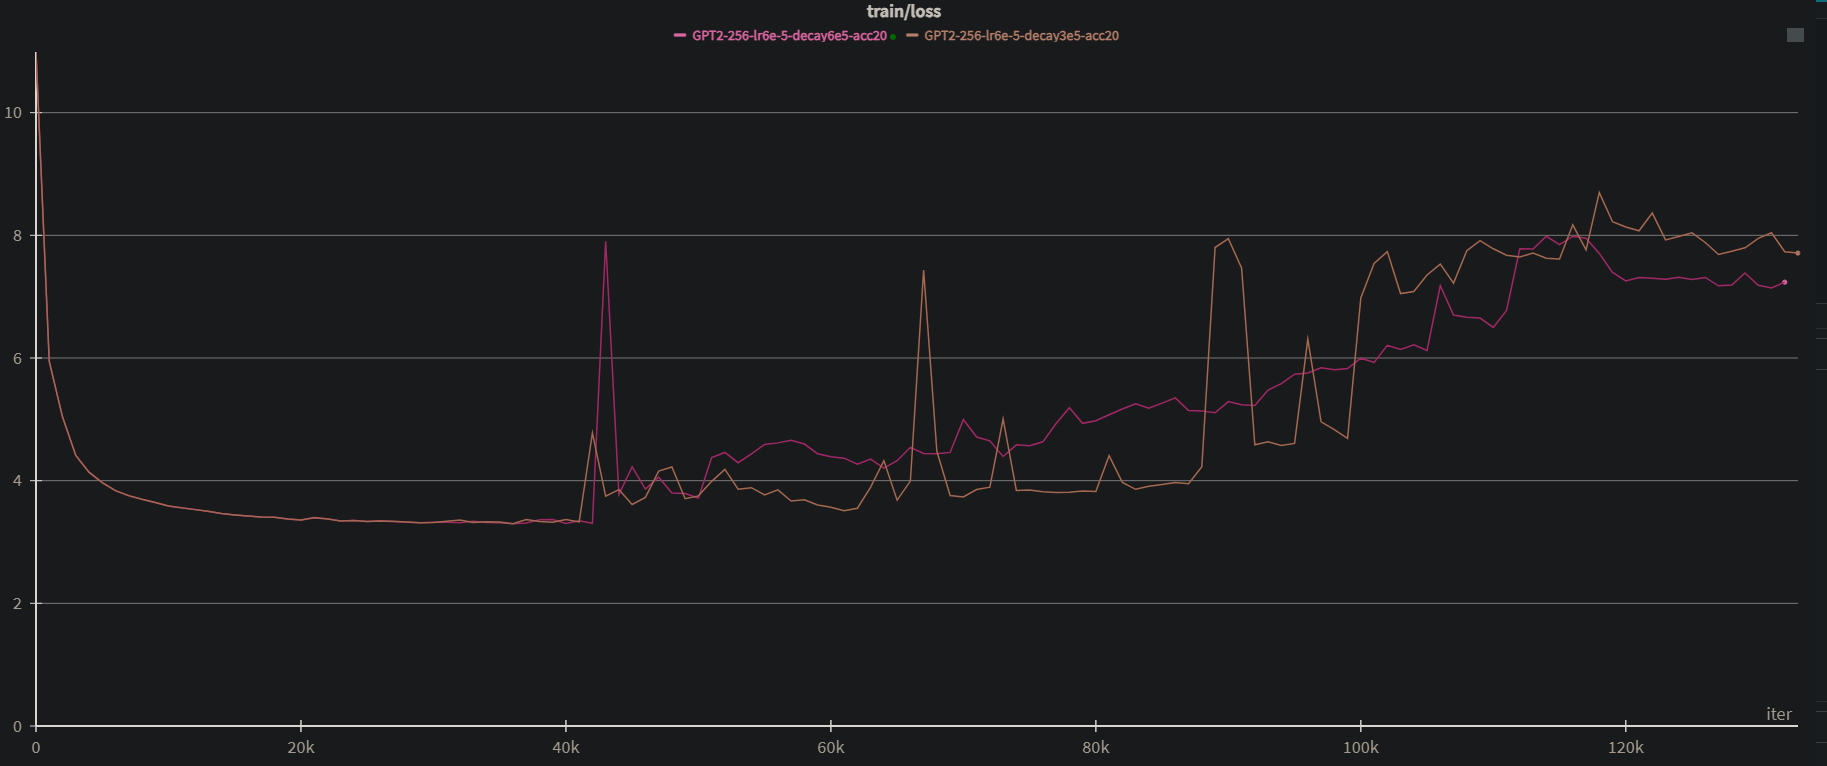
\includegraphics[width=\textwidth]{img/loss_in_nanogpt_524.png}  }
  \caption{nanoGPT 的 Github issue 中报告的两次独立 GPT-2 训练（BF16 + Flash Attention）损失曲线。}\label{fig:nanogpt_issues}
\end{figure}


\begin{figure}[t]
  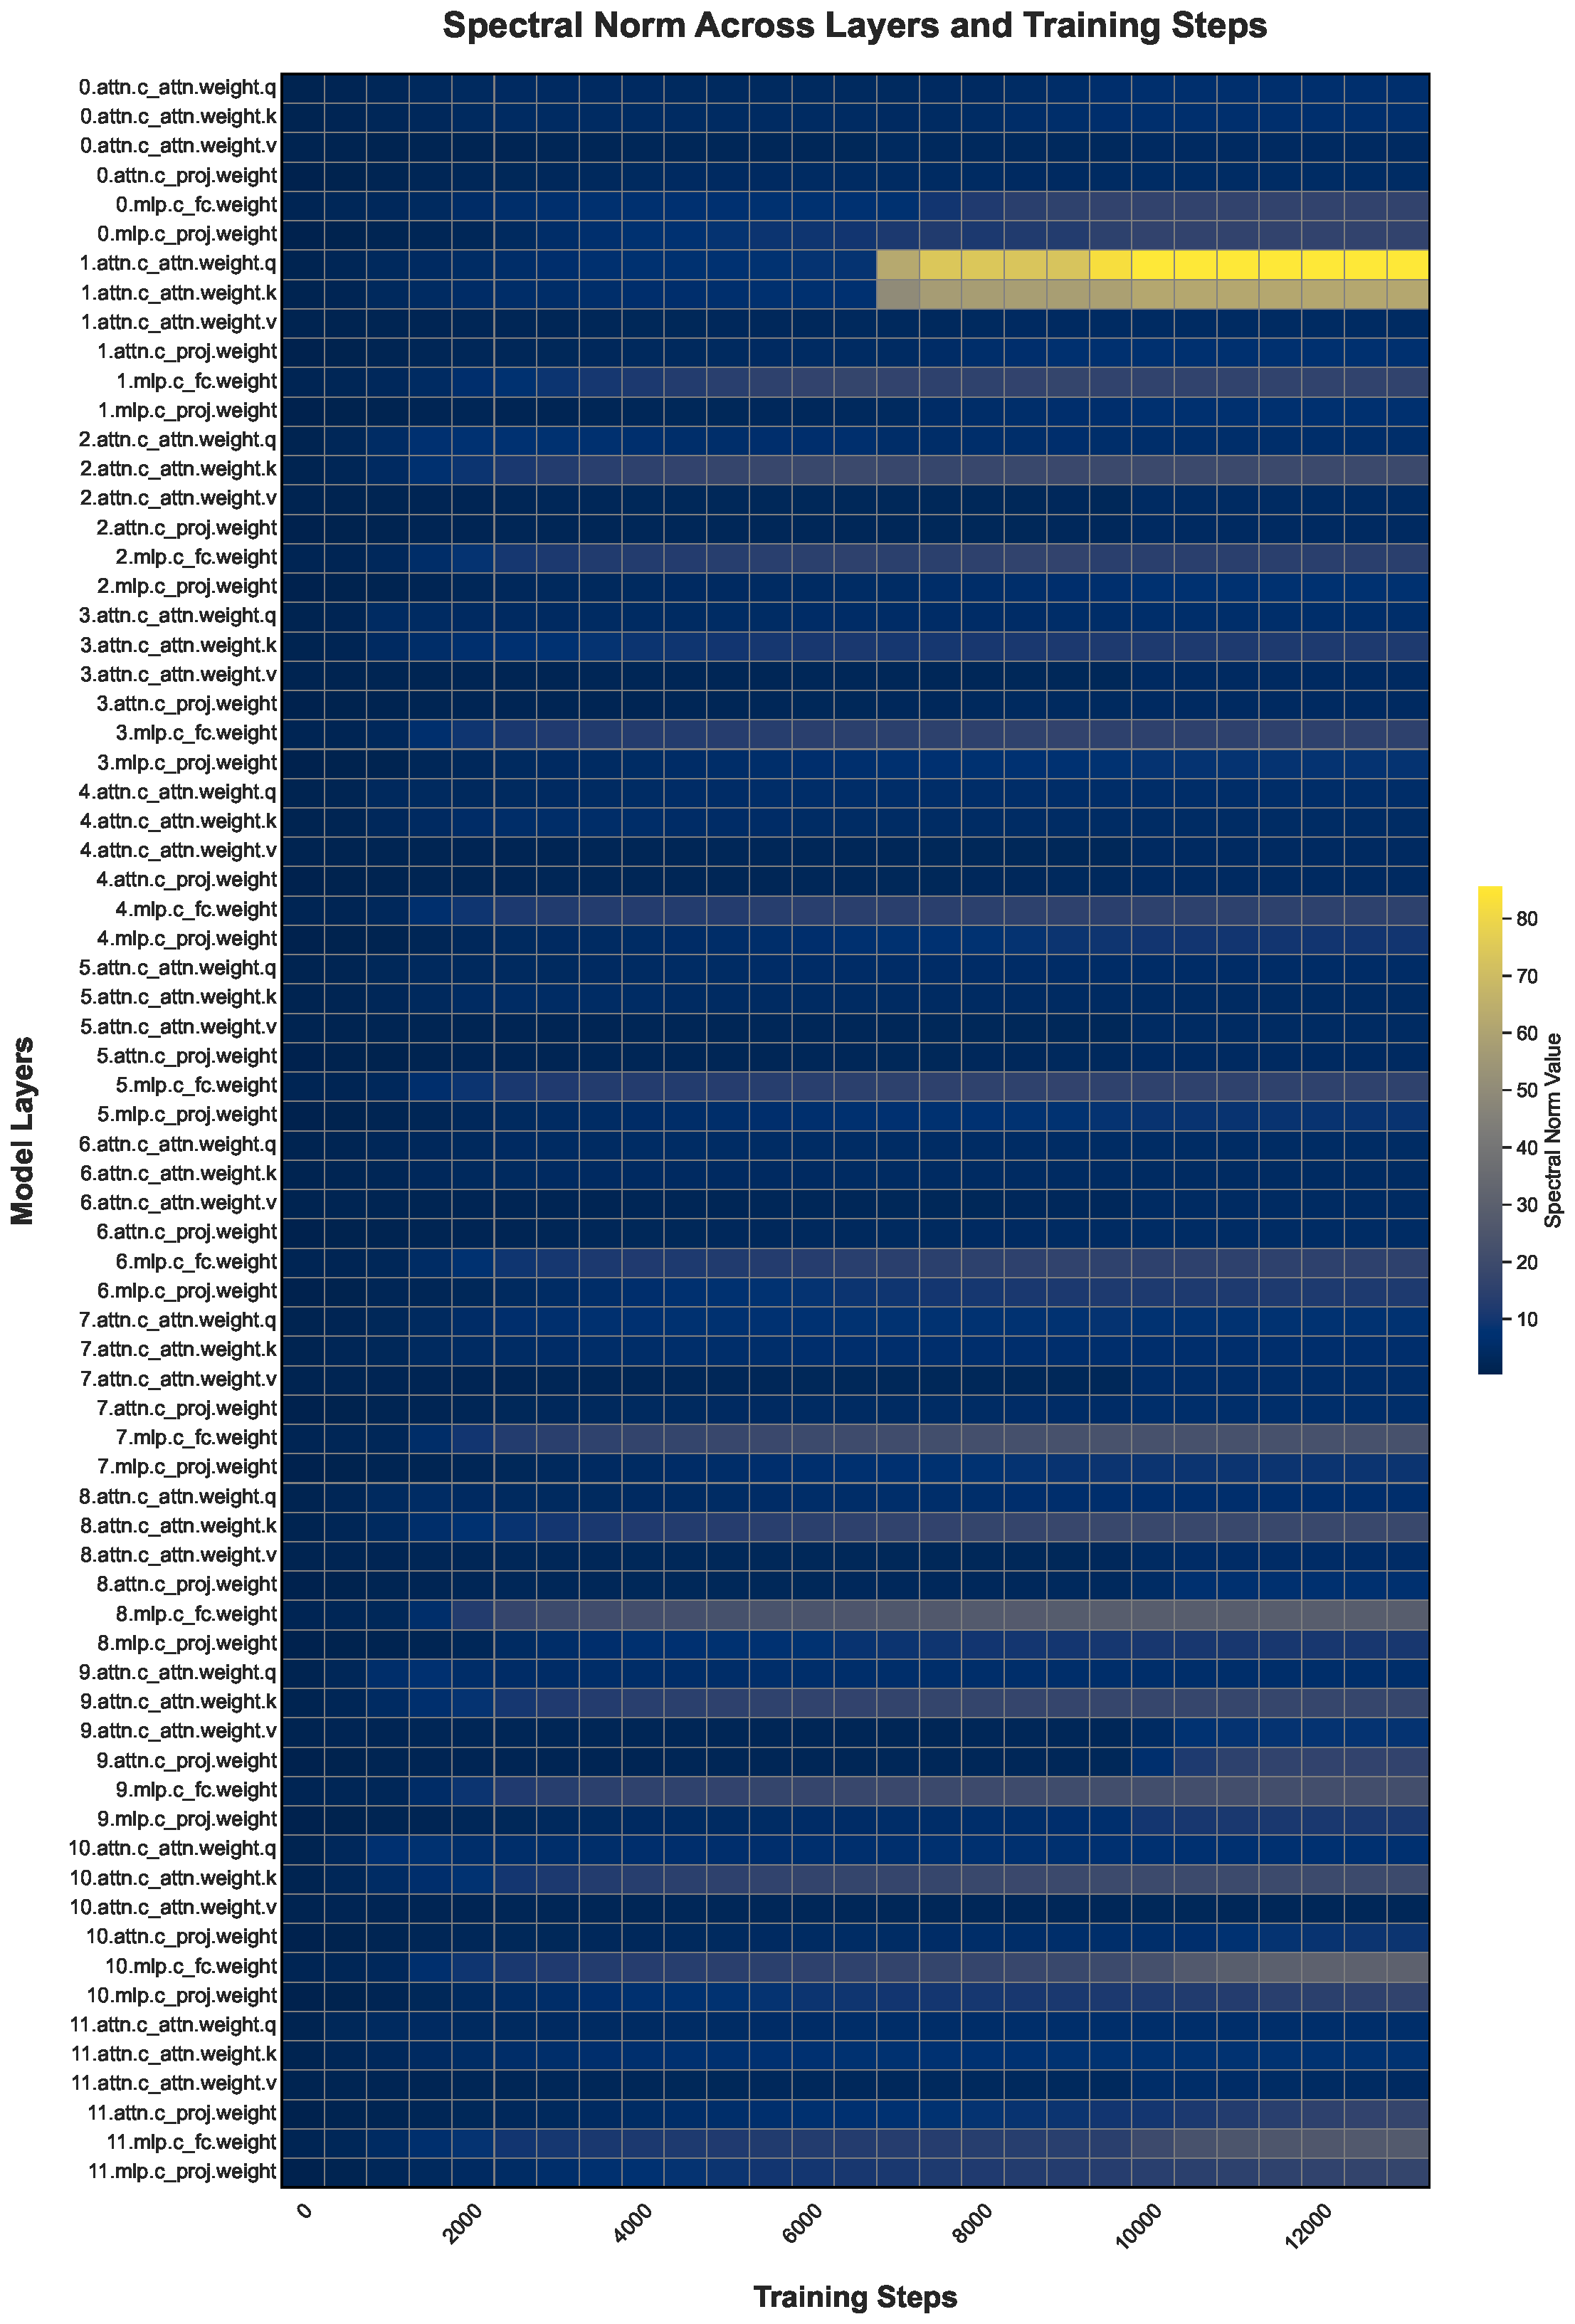
\includegraphics[width=\textwidth]{img/spectral_norm_heatmap.pdf}
  \caption{跨层与训练步骤的谱范数。}\label{fig:sp_norm}
\end{figure}


\begin{figure}[t]
  \centering
  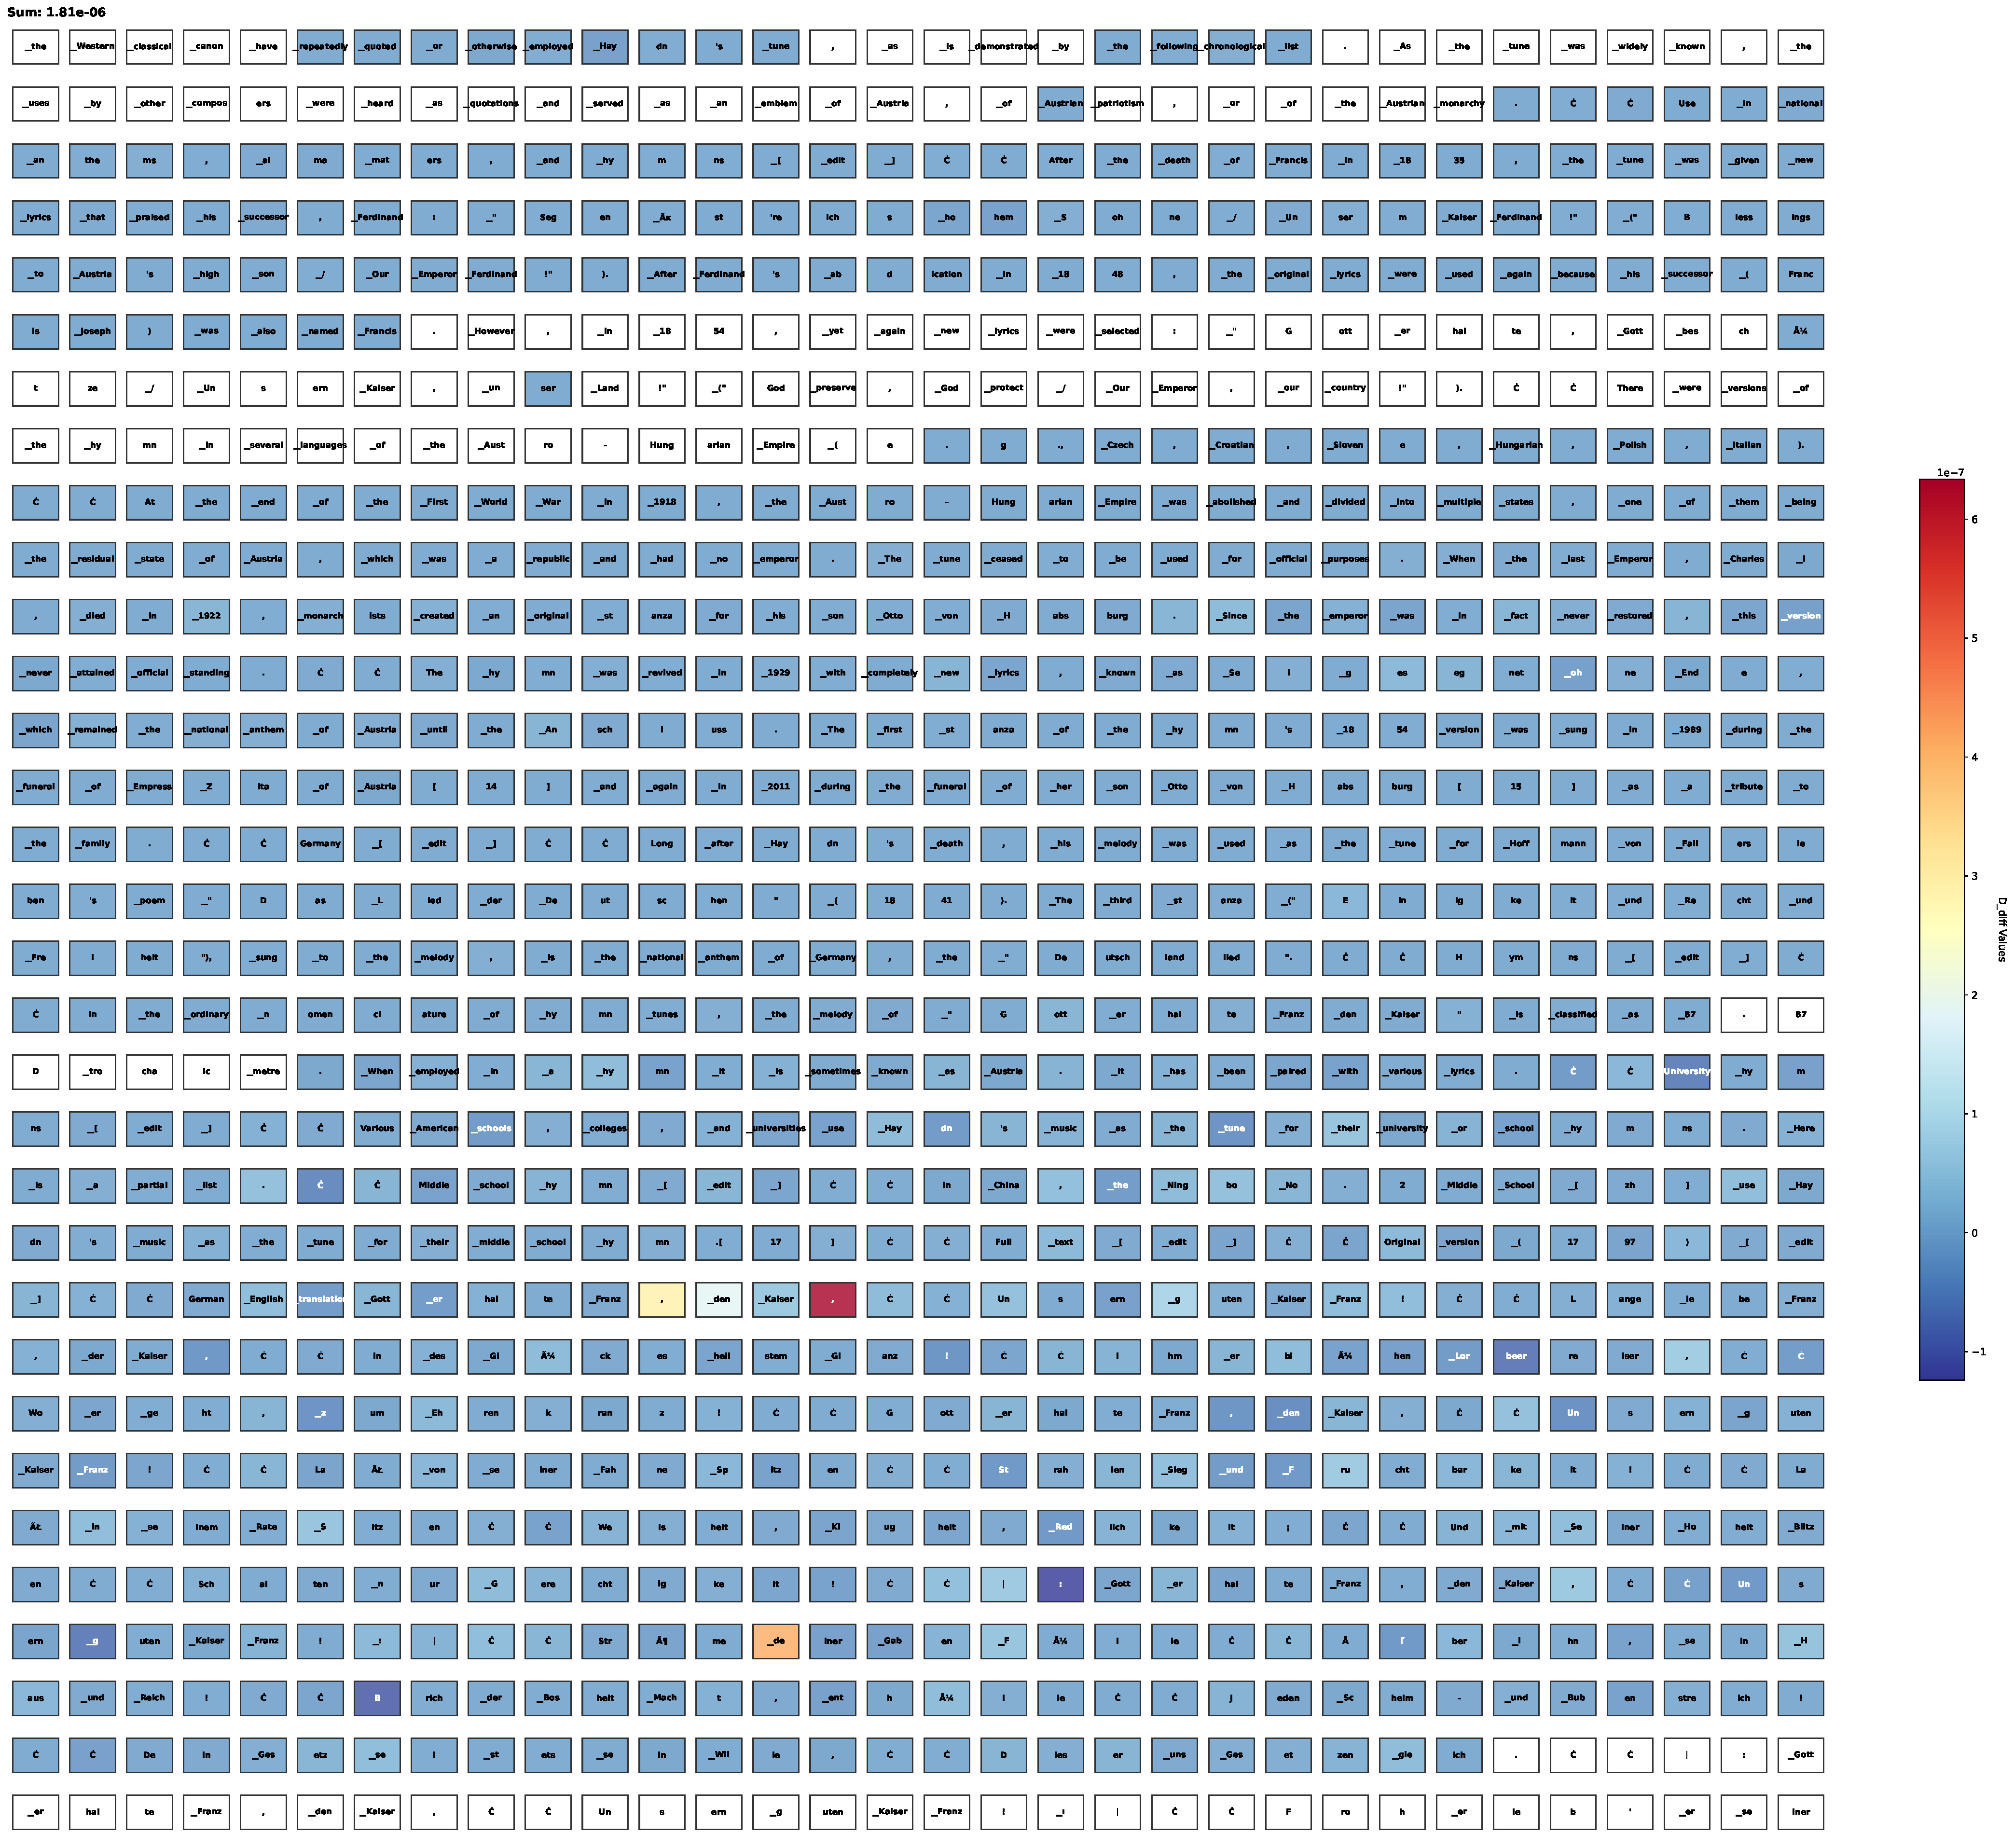
\includegraphics[width=\textwidth]{img/visualization_254.pdf}
  \caption{标记差异可视化}\label{fig:token_vis}
\end{figure}

\clearpage

\end{document}
